\chapter{Folgen und Reihen (Der Begriff des Limes)}
\section{Allgemeines zu Folgen}
\begin{definition}{3.1}
Eine Folge reeller Zahlen ist eine Abbildung $a:\N\backslash\{0\}\to\R$ wobei wir das Bild von $n\geq 1$ mit $a_n$ (statt $a(n)$) bezeichnen.\\

Eine Folge wird dann meistens mit $(a_n)_{n\geq 1}$, also mit der geordneten Bildmenge bezeichnet.
\end{definition}

\noindent  Folgen können auf verschiedene Arten gegeben sein.
\subsubsection*{Beispiel 3.2}
\begin{enumerate}
\item $a_n=\frac{1}{n}$, $n\geq 1$
\item $a_1=0.9$, $a_2=0.99$, \dots, ${a_n} = 0.\underbrace {99 \ldots 9}_{n-\text{mal}}$
\item $a_n=\left( 1+\frac{1}{n}\right)^n$, $n\geq 1$
\item (Rekursiv) Sei $d>0$ eine reelle Zahl. \\ $a_1,\dots, a_{n+1}:=\frac{1}{2}\left( a_n + \frac{d}{a_n}\right), n\geq 1$\\
z.B. $d=2,a_1=1,a_2=\frac{3}{2},a_3=\frac{17}{12},a_4=\dots$
\item Fibonacci Zahlen. $a_1=1,a_2=2, a_{n+1}=a_n+a_{n-1}\hspace{5mm}\forall n\geq 2$
\end{enumerate}

\begin{definition}{3.3}
Eine Folge $(a_n)_{n\geq 1}$ heisst beschränkt, falls die Teilmenge $\{a_n:n\geq 1\}\subseteq\R$ beschränkt ist. d.h. es gibt $c\in\R (c\geq 0)$, so dass $\abs{ a_n} \leq c, \forall n\geq 1$
\end{definition}

\section{Grenzwert oder Limes eine Folge. Ein zentraler Begriff}
\begin{definition}{3.4}
Eine Folge $(a_n)\geq 1$ konvergiert gegen $a$ wenn es für jedes $\varepsilon>0$ einen Index $N(\varepsilon)\geq 1$ gibt, so dass \[  \abs{ a_n-a} <\varepsilon, \forall n>N(\varepsilon)\]
\end{definition}

\begin{definition}{3.4 (Version 2)}Eine Folge $(a_n)_{n\geq 1}$ konvergiert gegen $a\in\R$, falls für jedes $\varepsilon>0$ die Menge der Indizes $n\geq 1$ für welcher $a_n\not\in (a-\varepsilon,a+\varepsilon)$ endlich ist.\\

\centerline{$\left( \forall\varepsilon>0, \#\{ n\in\N\mid a_n\not\in (a-\varepsilon,a+\varepsilon)\} <\infty\right)$}
\end{definition}

\beweis{der Äquivalenz beider Definitionen}
\begin{enumerate}

\item[(2)] $\Rightarrow(1)$ \\Sei für  $\varepsilon>0$ \[M(\varepsilon):=\{ n\in\N\mid a_n\not\in (a-\varepsilon,a+\varepsilon)\}=\{n\in\N\mid \abs{ a_n-a }\geq \varepsilon\}\]
Da $M(\varepsilon)$ endlich ist, ist es nach oben beschränkt. Es  gibt also $N(\varepsilon)\in\N$, so dass $\forall n\in M(\varepsilon)$, $n\leq N(\varepsilon)-1$. Insbesondere gilt $\forall n\geq N(\varepsilon)$, $n\not\in M(\varepsilon)$ und daher $\abs{ a_n-a}<\varepsilon$.
\item[(1)] $\Rightarrow(2)$ \[M(\varepsilon)=\{ n:\abs{ a_n-a} \geq \varepsilon\} \subset \left[ 0,N(\varepsilon)-1 \right]\] Also endlich.
\end{enumerate}

\noindent Falls die Eigenschaften in Definition 3.4 zutrifft, schreibt man\[a = \mathop {\lim }\limits_{n \to \infty } {a_n}{\text{ oder }}{a_n}\mathop  \to \limits_{n \to \infty } a\] Die Zahl $a$ nennt sich Grenzwert oder Limes der Folge $(a_n)_{n\geq 1}$. Eine Folge heisst konvergent falls sie einen Limes besitzt, andernfalls heisst sie divergent.

\subsubsection*{Bemerkung 3.5}
\begin{enumerate}
\item Falls $(a_n)_{n\geq 1}$ konvergiert, ist der Limes eindeutig bestimmt
\subsubsection*{Beweis}
Seien $a$ und $b$ Grenzwerte von $(a_n)_{n\geq 1}$. Sei $\varepsilon = \abs{ \frac{b-a}{3}}>0$, dann gibt es $N_1,N_2$, so dass \[\abs{ a_n-a} <\varepsilon\hspace{10mm}\forall n>N_1\]\[\abs{ a_n-b} <\varepsilon\hspace{10mm}\forall n>N_2\]
Also $\forall n\geq \max\{ N_1,N_2\}$ \[(a-b)\cong\abs{ (a-a_n)+(a_n-b)} < 2\varepsilon=\frac{2}{3}\abs{b-a}\]
\item Falls $(a_n)_{n\geq 1}$ konvergent ist, $\{a_n:n\geq 1\}$ beschränkt: Sei $\varepsilon=1$, $\lim a_n=a$ und $N_0$ mit \[\abs{ a_n-a} \leq 1\hspace{10mm} \forall n>N_0\] Dann ist $\forall n$ $\abs{ a_n} \geq \max\{\abs{ a} +1,\abs{ a_j}, 1\leq j\leq N_0  \}$
\end{enumerate}
\subsection*{Binomischer Lehrsatz}
Für beliebige Zahlen $a,b$ und $n\in\N$ ist \[{\left( {a + b} \right)^n} = \sum\limits_{k = 0}^n { {n \choose k} {a^{n - k}}{b^k}} \]
\subsubsection*{Beispiel 3.6}
\begin{enumerate}
\item Sei $a_n=\frac{1}{n}, n\geq 1$. Dann gilt $\lim a_n=0$
\begin{itemize}
\item Sei $\varepsilon>0$. Dann $\frac{1}{\varepsilon}>0$. Sei $n_0\in\N$, $n_0\geq 1$ mit $n_0>\frac{1}{\varepsilon}$ (Archimedische Eigenschaft, Satz 2.13)\\
\end{itemize}
Dann gilt für alle $n\geq n_0$, $\frac{1}{\varepsilon}<n_0\leq n \Rightarrow \abs{ \frac{1}{n}-0} = \frac{1}{n}<\varepsilon, \forall n\geq n_0$
\item Sei $0<q<1$ und $a_n:=q^n$, $n>1$. Dann gilt $\lim a_n=0$ ($a_n$ konvergiert gegen 0)
\subsubsection*{Beweis}
Zu beweisen \[\forall \varepsilon > 0, \exists N_0=N_0(\varepsilon)\in \N\]
\[\forall n\geq N_0:q^n <\varepsilon\]
Die Idee ist, zu zeigen, dass $\frac{1}{q^n}$ sehr gross wird und deswegen $q^n$ sehr klein wird. Setzen wir $\frac{1}{q}=1+\delta$ mit $\delta>0$ $\left( q<1\Rightarrow \frac{1}{q}>1\right)$%CHECK FROM HERE
 $$\frac{1}{q^n}=\left( \frac{1}{q}\right)^n=\left( 1+\delta\right)^n=1+n\delta + {n \choose 2} \delta^2+\dots+\delta^n\geq 1+n\delta>n\delta, \forall n\in\N$$
also \[0<q^n<\frac{1}{n\delta}, \forall n\in\N\]
Sei jetzt $\varepsilon >0$, wähle $N_0=N_0(\varepsilon)$ mit $\frac{1}{\varepsilon\delta}<N_0\Rightarrow \frac{1}{N_0\delta}<\varepsilon$
\[\forall n>N_0\hspace{5mm}0<q^n\leq\frac{1}{n\delta}<\frac{1}{N_0\delta}<\varepsilon\]
\item $a_{n}=\sqrt[n]{n}$, $\lim a_n=1$. Klar: $n\geq 1$ also $\sqrt[n]{n}\geq 1$\\
Gegeben ein $\varepsilon>0$, wollen wir $n$ so gross wählen, dass \[\sqrt[n]{n}-1 <\varepsilon\] das heisst, $n<\left( 1+\varepsilon \right)^n$. Wir entwickeln \[\left( 1+\varepsilon\right)^n=1+n\varepsilon+{n \choose 2} \varepsilon^2 + \dots +\varepsilon^n\]
$\varepsilon$ ist klein aber fixiert.\\

Für sehr grosse $n$ wird $1+n\varepsilon$ nie grösser als $n$ sein. Wir versuchen unser Glück mit dem Term ${n \choose 2} {\varepsilon ^2}$.
\[{n \choose 2} {\varepsilon ^2} = \frac{{n(n - 1)}}{2}\varepsilon^2 \] Wir benutzen also $( 1+\varepsilon )^n\geq \frac{n(n-1)}{2}\varepsilon^2$. Wir wollen $n$ so wählen, dass \[\frac{{n(n - 1)}}{2}{\varepsilon ^2} > n\] d.h. $n-1>\frac{2}{\varepsilon^2}$ oder $n>1+\frac{2}{\varepsilon^2}$\\

Setzen wir $N_0:=\left( 1+\frac{2}{\varepsilon^2}\right)+1$. Dann gilt für $\forall n>N_0$ \[(1+\varepsilon)^n > n \geq 1\]
\[\Rightarrow 1\leq \sqrt[n]{n}\leq 1+\varepsilon\]
\[\Rightarrow -\varepsilon<0\leq\sqrt[n]{n}-1\leq\varepsilon\Rightarrow \abs{ \sqrt[n]{n}-1} <\varepsilon, \forall n>N_0\]
\item Nicht alle Folgen sind konvergent. Es gibt zwei verschiedene Verhältnisse einer divergenten Folge \[a_n=(-1)^n \Rightarrow \{1,-1,\dots \}\text{ beschränkt aber nicht konvergent}\]
\item $a_n=n$ unbeschränkt, divergent.
\end{enumerate}

\subsubsection*{Beispiel 3.7}
Seien $p\in\N$, $0<q<1$. Dann gilt $\lim\limits_{n\to\infty}n^p q^n=0$. Das heisst, Exponentialfunktionen wachsen schneller als jede Potenz (wenn $x$ genügend gross ist, $a^x>x^b$)

\subsubsection*{Beweis}
Der Trick ist folgender \[{n^p}{q^n} = {\left( {{n^{\frac{p}{n}}} \cdot q} \right)^n} = {\left( {{{\left( {\sqrt[n]{n}} \right)}^p}{{\left( {{q^{\frac{1}{p}}}} \right)}^p}} \right)^n}\] Wir werden Beispiel 3.6 (2.),(3.) benutzen. \\(d.h. $\lim\sqrt[n]{n}=1 \hspace{10mm}\lim r^n=0, 0<r<1$) \\

Da $\lim\sqrt[n]{n}=1$, $\forall\eta >0$, $\exists N_0(\eta)$ \[\sqrt[n]{n}<1+\eta, n>N_0(\eta)\]
Wir wählen $\eta >0$, so dass ${q^{\frac{1}{p}}} = \frac{1}{{{{\left( {1 + \eta } \right)}^2}}}$. Dann
\[\sqrt[n]{n}\cdot q^{\frac{1}{p}}\leq\frac{\left( 1+\eta\right)}{\left( 1+\eta\right)^2}=\frac{1}{1+\eta}\hspace{10mm} \forall n>N_0\left(\eta\right)\]
Wobei \[\forall n>N_0\left(\eta\right)\]\[a_n=\left( \sqrt[n]{n}q^{\frac{1}{p}}\right)^{pn}<r^n\] mit \[r:=\left( \frac{1}{1+\eta}\right)^p, r<1\]
Sei jetzt $\varepsilon>0$. Da $\lim r^n=0$, $\exists N_1=N_1(\varepsilon)$, $\forall n>N_1(\varepsilon)$, $r^n<\varepsilon$\\

\noindent Für $n>\max\{N_0\left(\eta\right), N_1(\varepsilon)\}$, $a_n<r^n<\varepsilon \Rightarrow \lim a_n=\lim n^pq^n=0$

\section{Konvergenzkriterien}
Mit konvergenten Folgen kann man ``rechnen'' wie folgender Satz zeigt.
\subsubsection*{Satz 3.8}
Seien $\left( a_n\right)_{n\geq 1}$ und $\left( b_n\right)_{n\geq 1}$ konvergente Folgen mit
\[\lim a_n=a\text{, }\lim b_n=b\]
\begin{enumerate}[\hspace{2mm}i)]
\item Die Folge $\left( a_n+b_n\right)_{n\geq 1}$ konvergiert und $\lim\left( a_n+b_n\right)=a+b$
\item Die Folge $\left( a_n\cdot b_n\right)_{n\geq 1}$ konvergiert und $\lim\left( a_n\cdot b_n\right)=a\cdot b$
\item Falls $b\not=0$ und $b_n\not=0$ $\forall n\geq 1$, gilt $\lim\frac{a_n}{b_n}=\frac{a}{b}$
\item Falls $a_n\leq b_n$ folgt $a\leq b$
\end{enumerate}

\begin{beweis}{}
Sei $\varepsilon >0$, es gibt  $N_1(\varepsilon)$, $N_2(\varepsilon)$, so dass
\begin{align*}
\abs{ a_n-a}&<\varepsilon, \forall n>N_1(\varepsilon)\\
\abs{ b_n-b}&<\varepsilon, \forall n>N_2(\varepsilon)
\end{align*}
\begin{enumerate}[\hspace{2mm}i)]
\item Für $n\geq\max\left\{ N_1(\varepsilon),N_2(\varepsilon)\right\}$ gilt \[\abs{ {\left( {{a_n} + {b_n}} \right) - \left( {a + b} \right)} } \le \abs{ {{a_n} - a} } + \abs{ {{b_n} - b} }\]
Da dies für alle $\varepsilon>0<2\varepsilon$ gilt, folgt auch, dass
\[\forall n > \max \left\{ {{N_1}\left( {\frac{\varepsilon }{2}} \right),{N_2}\left( {\frac{\varepsilon }{2}} \right)} \right\}: = N(\varepsilon )\]
gilt \[\abs{ a_n+b_n-(a+b)} <\varepsilon\]
\item Sei $C$ eine Schranke für $\left\{ \abs{b_n} : n\geq 1\right\}$ (Bemerkung 3.5: Falls $\left( b_n\right)_{n\geq 1}$ konvergent ist, ist $\left\{b_n : n\geq 1\right\}$ beschränkt). Für $N_1(\varepsilon)$, $N_2(\varepsilon)$ wie oben folgt $\forall n\geq\max\left\{ N_1(\varepsilon), N_2(\varepsilon)\right\}$

\begin{align*}
\abs{ {{a_n}{b_n} - ab} } &=\abs{ {{a_n}{b_n} - a{b_n} + a{b_n} - ab} }\\
 &=\abs{ {{b_n}\left( {{a_n} - a} \right) + a\left( {{b_n} - b} \right)} }\\
 &\le \abs{ {{b_n}} }\varepsilon + \abs{ a }\varepsilon  \le \varepsilon \left( {C + \abs{ a }} \right)
\end{align*}

Aus \[\forall n \ge N(\varepsilon ): = \max \left( {{N_1}\left( {\frac{\varepsilon }{{C + \abs{ a }}}} \right),{N_2}\left( {\frac{\varepsilon }{{\abs{ C } + a}}} \right)} \right)\]
folgt, dass $\abs{ a_nb_n-ab} < \varepsilon$
\item Wegen (ii) genügt es, den Fall $a=a_n=1$, $\forall n\in\N$ zu betrachten
\[\abs{ {{b_n}} } = \abs{ {{b_n} - b + b} } \ge \abs{ b } - \abs{ {{b_n} - b} } \ge \abs{ b } - \varepsilon \]
Sei $0 < \varepsilon < \frac{\abs{ b}}{2}$, dann gilt $\abs{ b_n} > \frac{\abs{ b}}{2}$. Es folgt

\[\abs{ {\frac{1}{{{b_n}}} - \frac{1}{b}} } = \abs{ {\frac{{{b_n} - b}}{{{b_n}b}}} } < \frac{2}{{{{\abs{ b }}^2}}}\abs{ {{b_n} - b} } \le \frac{2}{{{{\abs{ b }}^2}}}\varepsilon \hspace{10mm}\forall n > {n_0}(\varepsilon )\]
Also folgt $\forall n > N(\varepsilon):=n_0\left( \frac{\varepsilon\abs{ b}^2}{2}\right)$ dass $\abs{ \frac{1}{b_n}-\frac{1}{b}} < \varepsilon$
\item (Indirekter Beweis) Falls $a>b$, $a-b>0$. Sei
\begin{align*}
\varepsilon&:= \frac{a-b}{2}>0\\
2\varepsilon&= b-a\\
\Rightarrow b-\varepsilon&= a+\varepsilon\\
b_n\to b\Rightarrow&b_n < b+\varepsilon\hspace{5mm}\forall n>n_0(\varepsilon)\\
a_n\to a\Rightarrow&-\varepsilon < a_n -a<\varepsilon\Rightarrow a-\varepsilon < a_n\hspace{5mm}\forall n> ??
\end{align*}
\todo{unreadble}
Jedoch steht dann die Ungleichung
\[b_n < b+\varepsilon = a-\varepsilon < a_n\hspace{5mm}\forall n\geq n_0\]
im Widerspruch zur Annahme $a_n\leq b_n$, $\forall n\in\N$
\end{enumerate}
\end{beweis}
Es ist nicht unbedingt nötig, den ganzen Beweis zu führen, um zu wissen, dass eine Folge konvergent ist. Es gibt Folgen, deren Konvergenz durch eine Strukturelle Eigenschaft gesichert ist, ohne dass man den Limes apriori kennen muss.\\

Folgender Satz illustriert das, er benützt das Vollständigkeitsaxiom
\subsubsection*{Satz 3.9 (Monotone Konvergenz)}\label{satz3.9}
\begin{enumerate}
\item Sei $\left( a_n\right)_{n > 1}$ eine monoton wachsende beschränkte Folge. Dann ist sie konvergent und es gilt zudem \[\mathop {\lim }\limits_{n \to \infty } {a_n} = \sup \left\{ {{a_n}:n \ge 1} \right\}\]
\item Sei $\left( b_n\right)_{n \geq 1}$ eine monoton fallende beschränkte Folge. Dann ist sie konvergent und es gilt zudem \[\mathop {\lim }\limits_{n \to \infty } {b_n} = \inf \left\{ {{b_n}\mid n \ge 1} \right\}\]
\end{enumerate}

\begin{definition}{3.10}
\begin{itemize}
\item \textbf{Monoton wachsend}: \[a_n\leq a_{n+1}\hspace{5mm}\forall n\geq 1\]
\item \textbf{Monoton fallend}: \[b_{n+1}\leq b_{n}\hspace{5mm}\forall n\geq 1\]
\end{itemize}
\end{definition}
\todo[inline]{Number might be wrong, page 63 middle}

\begin{beweis}{3.9}
\begin{enumerate}[\hspace{2mm}i)]
\item $a_1\leq a_2\leq \dots$ und $\left\{ a_n:n\geq 1\right\}$ nach oben beschränkt $\Rightarrow\exists C$ mit $a_n\leq C$ $\forall n\geq 1$. Sei nach Satz 2.9 (Jede nach oben beschränkte Teilmenge $A\subset R$ besitzt eine kleinste obere Schranke)   $a:=\sup \left\{ a_n:n\geq 1\right\}$ die kleinste obere Schranke. \\

Wir behaupten, dass: $a = \mathop {\lim }\limits_{n \to \infty } {a_n}$. Sei $\varepsilon>0$, dann ist $a-\varepsilon$ keine obere Schranke und deswegen gibt es $n(\varepsilon)\geq 1$ mit $a_{n(\varepsilon)}>a-c$. Aus der Monotonität folgt
\[a_n>a_{n(\varepsilon)} > a-c\hspace{5mm}\forall n>n(\varepsilon)\]
und damit folgt
\[ \abs{ a_n-a} < \varepsilon\hspace{5mm}\forall n> n(\varepsilon)\]
\item Ähnlich.
\end{enumerate}
\end{beweis}
Sätze 3.8, 3.9 haben vielfähige Anwendungen die wir durch einige Beispiele illustrieren.
\subsubsection*{Beispiel 3.10}
\begin{enumerate}
\item Sei \[{a_n} = \frac{{3{n^6} + 11{n^4} - 1}}{{2{n^6} - 7{n^3} + n}} = \frac{{3 + \frac{{11}}{{{n^2}}} - \frac{1}{{{n^6}}}}}{{2 - \frac{7}{{{n^3}}} + \frac{1}{{{n^5}}}}} \to \frac{3}{2}\]
\item $\mathop {\lim }\limits_{n \to \infty } {\left( {1 + \frac{1}{n}} \right)^n}$ existiert. \\

Wir werden beweisen, dass $a_n$ monoton wachsend und beschränkt ist. Dieser Limes wird mit ``$e$'' beteichnet, wobei $e=2.71828\dots$ (Eulersche Konstante)
\begin{beweis}{}
\[a_n={\left( {1 + \frac{1}{n}} \right)^n}\]
Wir möchten den binomischen Lehrsatz anwenden
\begin{align*}
{a_n} =&{\left( {1 + \frac{1}{n}} \right)^n}\\
=&1 + n\left( {\frac{1}{n}} \right) + \frac{{n(n - 1)}}{{2!}}{\left( {\frac{1}{n}} \right)^2} + \frac{{n(n - 1)(n - 2)}}{{3!}}{\left( {\frac{1}{n}} \right)^3} +  \ldots  + {\left( {\frac{1}{n}} \right)^n}\\
=&1 + 1 + \frac{1}{{2!}}\left( {1 - \frac{1}{n}} \right) + \frac{1}{{3!}}\left( {1 - \frac{1}{n}} \right)\left( {1 - \frac{2}{n}} \right)\\
&+\ldots  + \frac{1}{{k!}}\left( {1 - \frac{1}{n}} \right)\left( {1 - \frac{2}{n}} \right) \ldots \left( {1 - \frac{{k - 1}}{n}} \right) +  \ldots
\end{align*}
Nun ist aber
\begin{align*}
\frac{1}{{2!}}\left( {1 - \frac{1}{n}} \right)&< \frac{1}{{2!}}\left( {1 - \frac{1}{{n + 1}}} \right)\\
\frac{1}{{3!}}\left( {1 - \frac{1}{n}} \right)\left( {1 - \frac{2}{n}} \right)&< \frac{1}{{3!}}\left( {1 - \frac{1}{{n + 1}}} \right)\left( {1 - \frac{2}{{n + 1}}} \right)\\
&\text{usw}
\end{align*}
deswegen folgt \[2 < a_n < a_{n+1}\hspace{5mm}\forall n\geq 1\]
d.h. $a_n$ ist monoton wachsend.\\

\noindent Die Produkte der Form
\begin{align*}
\left( {1 - \frac{1}{n}} \right) &\ldots \left( {1 - \frac{{k - 1}}{n}} \right) < 1\\
 \Rightarrow {a_n} &< 1 + 1 + \frac{1}{{2!}} + \frac{1}{{3!}} +  \ldots \\
&< 1 + 1 + \frac{1}{2} + \frac{1}{{{2^2}}} + \frac{1}{{{2^3}}} \ldots  = 3
\end{align*}
d.h. $a_n$ ist beschränkt. Monotone Konvergenz $\Rightarrow \left( a_n\right)_{n\geq 1}$ konvergiert
\end{beweis}
\item Rekursive Definitionen\\
Sei $\mathop {c > 1}\limits_{c \in\R }$, $a_1=c$, ${a_{n + 1}} = \frac{1}{2}\left( {{a_n} + \frac{c}{{{a_n}}}} \right)$, $n\geq 1$. Dann ist $\lim a_n=\sqrt{c}$
\begin{beweis}{}
Dies ist ein wichtiges Beispiel. Hier wird vorgeführt wie man aus der apriori Existenz des Limes dessen Wert schliessen kann.\\

\noindent\underline{1. Schnitt:}
\[a_{n + 1}^2 \ge c\hspace{5mm}\forall n\geq 1\]
$a_n$ ist (nach unten) beschränkt.
\begin{align*}
{a_{n + 1}} =&\frac{{c + a_n^2}}{{2an}} = {a_n} + \frac{{c - a_n^2}}{{2{a_n}}}\\
 \Rightarrow a_{n + 1}^2 =&a_n^2 + \left( {c - a_n^2} \right) + {\left( {\frac{{c - a_n^2}}{{2{a_n}}}} \right)^2}\\
 =&c + {\left( {\frac{{c - a_n^2}}{{2{a_n}}}} \right)^2} \ge c\hspace{2mm}\text{(\textasteriskcentered)}
\end{align*}
\noindent\underline{2. Schnitt:}
\[a_{n+1}\leq a_n\]
d.h. $a_n$ ist monoton fallend.
\begin{align*}
\text{(\textasteriskcentered)}: a_{n+1}^2&\geq c\\
\Rightarrow\frac{c}{a_{n+1}}&\leq a_{n+1}\hspace{5mm} \forall n\in\N\text{, insbesondere}\\
\frac{c}{a_n}&\leq a_n \\
\Rightarrow a_{n+1}&=\frac{1}{2}\left( {{a_n} + \frac{c}{{{a_n}}}} \right) \le \frac{1}{2}\left( {{a_n} + {a_n}} \right) = {a_n}
\end{align*}
Mit dem Satz der monotonen Konvergenz folgt, dass $\left( a_n\right)$ konvergiert.\\

\noindent Sei $a=\lim a_n$. Da $a_n^2\geq c$, $\forall n\geq 2$ folgt $a^2\geq c$. Aus $a_{n+1}=\frac{1}{2}\left( a_n+\frac{c}{a_n}\right)$ und Satz 3.8 folgt $a=\frac{1}{2}\left( a+\frac{c}{a}\right)$ $\Rightarrow\frac{c}{a}=a\Rightarrow c=a^2\Rightarrow a=\sqrt{c}$. Schliesslich $\lim a_n=\sqrt{c}$
\end{beweis}
\end{enumerate}

\section{Teilfolgen, Häufungspunkte}
\begin{definition}{3.11}
Sei $\left( a_n\right)_{n\in\N}\subset\R$ eine Folge und sei $l(n)_{n\in\N}$ eine strikt monoton wachsende Folge von positiven natürlichen Zahlen. Die Verkettung von $l(n)$ und $\left( a_n\right)$ heisst eine Teilfolge $\left( a_{l(n)}\right)_{n\in\N}$ von $\left( a_{n}\right)_{n\in\N}$
\[n\to l(n)\to a_{l(n)}\]
\end{definition}
Die Idee ist sehr einfach: Wir haben die Folge \[a_1,a_2,a_3,a_4,a_5,a_6,\dots,a_j,\dots,a_{j+1},\dots \]
und wir definieren eine neue Folge mit einigen Elementen von $\left( a_n\right)$
\[a_1,a_3,a_6,a_{j+1},\dots \]

\subsubsection*{Beispiele}
\begin{enumerate}
\item \begin{align*}
{a_n} =&\left\{ {1,0, - 1,1,0, - 1,1,0, - 1, \ldots } \right\}\\
 =&\left\{ {\begin{array}{*{20}{c}}
0&{{\text{falls}}}&{n = 3k + 2}\\
1&{{\text{falls}}}&{n = 3k + 1}\\
{ - 1}&{{\text{falls}}}&{n = 3k + 3}
\end{array}} \right.
\end{align*}
\begin{align*}
n&\to 3n + 2 \to {a_{3n + 2}} = \left( {0,0, \ldots } \right)\\
n&\to 3n + 1 \to {a_{3n + 1}} = \left( {1,1, \ldots } \right)\\
n&\to 3n \to {a_{3n}} = \left( { - 1, - 1, \ldots } \right)
\end{align*}
\item $\left( a_n\right)_{n\in\N}$, $a_n=n\Rightarrow \left( 2^n\right)_{n\in\N}$ ist eine Teilfolge $n\to 2^n\to a_{2^n}$
\item $a_n=\left( -1\right)^n$, $\left( a_{2n}\right)_{n\geq 1}$ $\left( a_{2n+1}\right)$ sind Teilfolgen
\end{enumerate}

\subsubsection*{Bemerkung 3.12}
In Definition 3.11 ist $l\left( \N\backslash\{ 0\}\right)$ eine unendliche Teilmenge von $\N\backslash\{ 0\}$. Umgekehrt, falls $\wedge\subset\N\backslash\{ 0\}$ eine unendliche Teilmenge ist, erhält man eine Teilfolge von $\left( a_n\right)_{n\geq 1}$ mittels einer monotonen Abzählung $l:\N\backslash\{ 0\}\to\wedge$ von $\wedge$ ($l(n):=\min\left( \wedge \backslash\{ l(1),l(2),\dots ,l(n-1)\}\right)$)
\begin{definition}{3.13}
$a\in\R$ ist Häufungspunkt von $\left( a_n\right)_{n\geq 1}$ falls es eine gegen $a$ konvergierende Teilfolge $\left( a_{l(n)}\right)_{n\geq 1}$ gibt.
\end{definition}
\subsubsection*{Beispiel 3.14}
\todo[inline]{Looks like there is no number 2, removed list in its entirety, page 71 middle to top}
$a_n=(-1)^n$ hat +1 und -1 als Häufungspunkte. Wir werden jetzt die Menge der Häufungspunkte einer Folge $\left( a_n\right)_{n\geq 1}$ näher studieren und insbesondere zeigen, dass sie für beschränkte Folgen nicht leer ist. \\

Sei $\left( a_n\right)_{n\geq 1}$ beschränkt und $C$ eine obere Schranke für $\{ \abs{ a_n} : n\geq 1\}$. Für jedes $k\geq 1$ ist die Menge
\[A_k:=\left\{ a_n:n\geq k\right\} = \left\{ a_k,a_{k+1},\dots\right\} \] beschränkt und zudem gilt \[A_{k+1}\subset A_k\text{, }\forall k\geq 1\]
Sei also
\begin{itemize}
\item $m_k:=\inf A_k \nearrow\left( \inf A_k < \inf A_{k+1}\right)$
\item $M_k:=\sup A_k\searrow\left( \sup A_{k+1} < \sup A_k\right)$
\end{itemize}
Dann folgt aus Korollar 2.11
\begin{enumerate}[\hspace{2mm}i)]
\item $\left( m_k\right)_{k\geq 1}$ monoton wachsend
\item $\left( M_k\right)_{k\geq 1}$ monoton fallend
\end{enumerate}
Nach dem Satz der monotonen Konvergenz (Satz 3.9, s.~\pageref{satz3.9}) konvergieren beide Folgen

\begin{definition}{3.15}
Wir definieren
\begin{itemize}
\item $\mathop {\lim }\limits_{n \to \infty } \inf {a_n}: = \mathop {\lim }\limits_{k \to \infty } {m_k}$, limes inferior
\item $\mathop {\lim }\limits_{n \to \infty } \sup {a_n}: = \mathop {\lim }\limits_{k \to \infty } {M_k}$, limes superior
\end{itemize}
Offensichtlich gilt $\lim\inf a_n\geq \lim\sup a_n$
\end{definition}
\noindent Interessant ist nun:
\subsubsection*{Lemma 3.16}
Sei $\left( a_n\right)_{n\geq 1}$ beschränkt. Dann sind $\lim\sup a_n$ und $\lim\inf a_n$ Häufungspunkte von $\left( a_n\right)_{n\geq 1}$

\begin{beweis}{}
Sei $\mathop {\lim }\limits_{n \to \infty } \sup {a_n} = a$. Wir möchten zeigen, dass eine Teilfolge $a_{l(n)}$ gibt mit $\lim a_{l(n)}=a$. Wir definieren $l:\N\backslash\{ 0\}\to\N\backslash\{ 0\}$ Induktive wie folgt:\\

\noindent $l(1)\geq 1$ sei so gewählt, dass $M_1-1\leq a_{l(1)}\leq M_1=\sup A_1=\{ a_1,a_2,\dots\}$
\begin{framed}
\noindent\textbf{Korollar 2.11}\\
Sei $h\in\R$, $h>0$
\begin{enumerate}
\item[4.] Falls $E$ ein $\sup$ besitzt $\Rightarrow\exists x\in E$ mit $x>\sup E-h$
\end{enumerate}
Sei $E=\{ a_1,\dots\}=A_1$, $h=1$
\end{framed}
Sei $l(2)\in\{ k\in\N\mid k>l(1)+1\}$, so dass \[M_{l(1)+1}\leq a_{l(2)}\leq M_{l(1)+1}\]
(Sei $E=\{ a_{l(1)+1},a_{l(1)+2},\dots\}$, $h=\frac{1}{2}$). Falls $l(1),l(2),\dots,l(n-1)$ definiert ist, wählen wir $l(n)$, so dass:
\[ l(n)\in\{ k\in\N : k>l(n-1)+1\}\]
und
\[
M_{l(n-1)+1}-\frac{1}{n}\leq a_{l(n)}\leq M_{l(n-1)+1}\tag{\text{\textasteriskcentered}}
\]
\[ \abs{ M_{l(n-1)+1}-a_{l(n)}} < \frac{1}{n}\]
Dann ist $l(n)$ strikt monoton steigend und
\[ \abs{ a_{l(n)} -M_{l(n-1)+1}}\leq\frac{1}{n}\]
Sei nun $\varepsilon > 0$ und $n(\varepsilon)$ so gewählt, dass $\frac{1}{n(\varepsilon)}<\frac{\varepsilon}{2}$ und
\[a-\frac{\varepsilon}{2}\leq M_{l\left( n(\varepsilon)-1\right) +1}\leq a+\frac{\varepsilon}{2} \]
($a=\lim M_k$: d.h. $\forall\varepsilon>0$, $\exists N(\varepsilon)$, so dass $\abs{ M_n -a} < \frac{\varepsilon}{2}$ $\forall n > N(\varepsilon)$). Dann gilt $\forall n > n(\varepsilon):\frac{1}{n}<\frac{\varepsilon}{2}$
\[\abs{ M_{l(n-1)+1} - a} < \frac{\varepsilon}{2}\tag{\text{\textasteriskcentered\textasteriskcentered}}\]
und
\[\abs{ M_{l(n-1)+1} - a_{l(n)}} < \frac{1}{n}< \frac{\varepsilon}{2}\tag{\text{\textasteriskcentered}}\]
(\textasteriskcentered) und (\textasteriskcentered\textasteriskcentered) $\Rightarrow\abs{ a_{l(n)}-a} < \varepsilon$ d.h. $\lim a_{l(n)}=a.$
\end{beweis}
Wir schliessen aus Lemma 3.16 den folgenden wichtigen Satz
\subsubsection*{Satz 3.18 (Bolzano - Weierstrass)}
Jede Beschränkte Folge $\left( a_n\right)_{n\geq 1}$ besitzt eine konvergente Teilfolge.
\todo[inline]{MISSING CONTENT: Can't really understand the layout of this part, page 76 middle}
Folgende Aussagen sind direkte Konsequenzen
\subsubsection*{Satz 3.19}
Sei $\left( a_n\right)_{n\geq 1}\subset\R$ beschränkt. $a_{-}:=\lim\inf a_n$, $a_+:=\lim\sup a_n$
\begin{enumerate}
\item $\forall\varepsilon > 0$ gibt es nur endlich viele $n\in\N$ mit $a_n\not\in\left( a_- -\varepsilon,a_+ +\varepsilon\right)$
\item $a_+$ ist der grösste, $a_-$ der kleinste Häufungspunkt
\item Folgende Aussagen sind äquivalent
\begin{enumerate}[(i)]
\item $\left( a_n\right)_{n\geq 1}$ konvergiert
\item Jede Teilfolge von $\left( a_n\right)_{n\geq 1}$ konvergiert
\item $a_-=a_+$
\end{enumerate}
\end{enumerate}
\subsubsection*{Bemerkung}
$\left( a_n\right)$ konvergiert gegen $a\Rightarrow$ jede Teilfolge konvergiert gegen $a$. Das ist ein sehr nutzliches Kriterium für Konvergenz

\subsubsection*{Beispiel 3.20}
Wir definieren rekursiv
\begin{align*}
g_1&=1, g_{n+1}=1+\frac{1}{g_n}, n\geq 1\\
g_1&=1, g_2=2, g_3=\frac{3}{2}, g_4=\frac{5}{3}
\end{align*}
\begin{center}
\begin{tikzpicture}[]
\draw 
(0,0) --(8,0)
(2,0.15) -- (2,-0.15)
(2,-0.1) node[anchor=north] {$1=g_1$}
(3,0.15) -- (3,-0.15)
(3,0.1) node[anchor=south] {$g_3$}
(5,0.15) -- (5,-0.15)
(5,0.1) node[anchor=south] {$g_4$}
(6,0.15) -- (6,-0.15)
(6,-0.1) node[anchor=north] {$2=g_2$};
\node[circle,fill=black,inner sep=0.5mm] (a) at (4,0) {};
\end{tikzpicture}
\end{center}
So die Folge ist nicht monoton. Offensichtlich gilt $g_n\geq 1$ und damit auch $g_n\leq 2$ d.h. $g_n$ ist beschränkt.\\

Aber wir werden werden zwei monotone Teilfolgen finden
\begin{align*}
{g_{n + 2}}&= 1 + \frac{1}{{{g_{n + 1}}}} = 1 + \frac{1}{{1 + \frac{1}{{{g_{n}}}}}}\\
&= \frac{2 + \frac{1}{g_{n}}}{1 + \frac{1}{{{g_{n}}}}} = \frac{2{g_{n} + 1}}{g_{n}+1} = 2 - \frac{1}{{{g_n} + 1}}
\end{align*}
Daraus folgt
\[{g_{n + 2}} - {g_n} = \frac{1}{{{g_{n - 2}} + 1}} - \frac{1}{{g_n} + 1} = \frac{g_{n} - g_{n - 2}}{{\left( {{g_{n - 2}} + 1} \right)\left( {{g_n} + 1} \right)}}\]
Nun ist: $g_3-g_1 = \frac{3}{2}-1>0$ und somit ist $g_{2k+3}-g_{2k+1}>0$, $\forall k$ d.h. die Teilfolge $\left( g_{2k+1}\right)_{k\geq 0}$ ist monotone wachsend.\\

\noindent$g_4-g_2=\frac{5}{3}-2<0$ woraus folgt, dass $\left( g_{2k}\right)_{k\geq 1}$ monoton fallend ist. Seien also
\begin{align*}
a&:=\lim_k g_{2k+1}\\
b&:=\lim_k g_{2k}
\end{align*}
Dann
\begin{align*}
a&:=\lim_k g_{2k+1}=\lim\left( 1+\frac{1}{g_{2k}}\right)\\
&=1+\frac{1}{b}\Rightarrow ab=b+1
\end{align*}
und analog $b=1+\frac{1}{a}\Rightarrow ab=1+a$ woraus $ab=1+a=b+1$ und somit $a=b$. Folgt mit $g:=a=b$ $g=1+\frac{1}{g}$ $\Rightarrow g=\frac{1+\sqrt{5}}{2}$\\

$g_+:=\lim\sup g_n$ und $g_-:=\lim\inf g_n$ sind Häufungspunkte, d.h. es gibt Teilfolgen $a_n$ und $b_n$ mit $\lim a_n=g_+$, $\lim b_n=g_-$. Da jede Teilfolge von $\left( g_n\right)$ entweder unendlich viele gerade oder ungerade Indizes enthält, folgt
\[g=g_+=g_-\]

\[
\sbox{\tempbox}{%
  $\displaystyle
    \begin{drcases}
    g_+ = \lim {a_n} = \lim g_{2n} = g\\
    g_+ = \lim {b_n} = \lim g_{2n} = g
    \end{drcases} 
    g_+ = g_- \Rightarrow \lim g_n = g = g_- = g_+ = \frac{1 + \sqrt{5}}{2}
  $%
}
\begin{pmatrix}
\,\parbox[b]{\wd\tempbox}{
  Jede Teilfolge hat entweder unendliche viele Elemente von
  $(g_{2n})$ oder $(g_{2n+1})$.
}\hfill\, % left alignment
\\[\abovedisplayskip]
\,\usebox{\tempbox}\,
\vspace{2mm}
\end{pmatrix}
\]

\section{Cauchy-Kriterium}
\todo[inline]{Chapter numbering is, according to the handwritten notes, wrong. WHich one is the correct one??}
\subsubsection*{Frage}
Wie sieht man allgemein, ob eine Folge konvergiert? Sei $\left( a_n\right)_{n\geq 1}$ konvergent mit $\lim a_n=a$. Also gibt es zu jedem $\varepsilon>0$, $n(\varepsilon)$ mit $\abs{ a_n-a}<\varepsilon$ $\forall n\geq n(\varepsilon)$ .\\
Daraus folgt, dass $\forall n,m\geq n(\varepsilon)$
\begin{align*}
\abs{a_n-a_m}&= \abs{ a_n-a+a-a_m}\\
&\leq \abs{ a_n-a }+\abs{ a_m-a} < 2\varepsilon
\end{align*}
\begin{definition}{3.21}
$\left( a_n\right)_{n\geq 1}$ ist eine Cauchy-Folge falls für $\varepsilon>0$ ein $n(\varepsilon)\geq 1$ gibt, so dass $\abs{ a_n-a_m}<\varepsilon$, $\forall n,m\geq n(\varepsilon)$
\end{definition}
Wir haben gesehen, dass
\[ \left( a_n\right) \text{ konvergiert }\Rightarrow\left( a_n\right) \text{ Cauchy}\]
Wir haben auch\todo{limenet: what??}
\subsubsection*{Satz 3.22 (Cauchy-Kriterium)}\label{satz3.22}
Sei $\left( a_n\right)_{n\geq 1}\subset\R$ eine Folge. Die folgenden Aussagen sind äquivalent
\begin{enumerate}
\item $\left( a_n\right)$ ist eine Cauchy-Folge
\item $\left( a_n\right)$ ist konvergent
\end{enumerate}

\begin{beweis}{}
\begin{enumerate}[align=left]
\item[$(2)\Rightarrow(1)$]\checkmark
\item[$(1)\Rightarrow(2)$] Wegen das Satzes von Bolzano - Weierstrass besitzt jede beschränkte Folge eine konvergente Teilfolge  \\

\underline{Strategie:}
\begin{enumerate}[I)]
\item $\left( a_n\right)$ beschränkt
\item $\exists\left( a_{l(n)}\right)\subset \left( a_n\right)$ konvergente Teilfolge
\end{enumerate}
Sei $\lim a_{l(n)}=a$, $\left( a_n\right)$ Cauchy.
\begin{align*}
\abs{a_n-a}&= \abs{ a_n-a_{l(n)}+a_{l(n)}-a}\\
&\leq \abs{ a_n-a_{l(n)} }+\abs{ a_{l(n)}-a} < 2\varepsilon
\end{align*}

\begin{enumerate}[I)]
\item $\left(a_n\right)$ ist beschränkt: Sei $\varepsilon=1$. Sei $n(1)$, so dass $\abs{ a_n-a_m}<1$, $\forall n,m\geq n(1)$, insbesondere $\abs{ a_n-a_m}<1$. Woraus $\abs{ a_n} < a_{n(1)}+1$, $\forall n\geq n(1)$ folgt und somit $\forall n\geq 1$
\[\abs{ {{a_n}} } \le \max \left\{ {\abs{ {{a_1}} }, \ldots ,\abs{ {{a_{n(1)}}} },\abs{ {{a_{n(1)}}} } + 1} \right\}\]
d.h. $\left( a_n\right)$ ist beschränkt
\item Sei $a$ ein Häufungspunkt von $\left( a_n\right)$ (Bolzano - Weierstrass) und $l:\N\to\N$ strikt monoton mit
\[\mathop {\lim }\limits_{n \to \infty } {a_{l(n)}} = a\hspace{10mm}\left( {{\text{Bem.: }}l(n) \ge n} \right)\]
\end{enumerate}
Sei $\varepsilon>0$ und $n_0(\varepsilon)$, so dass
\[\abs{ {{a_{l(n)}} - a} } < \varepsilon \hspace{10mm}\forall n > {n_0}(\varepsilon )\]
Sowie $n_1(\varepsilon)$ mit \\\todo{Can't understand, page 83 bottom}

$\forall n \ge \max \left\{ {{n_0}(\varepsilon ),{n_1}(\varepsilon )} \right\}$ gilt:
\begin{align*}
\abs{ {{a_n} - a} } &\le \abs{ {{a_n} - {a_{l(n)}}} } + \abs{ {{a_{l(n)}} - a} }\\
&\le \varepsilon  + \varepsilon  = 2\varepsilon
\end{align*}
\[ \Rightarrow \lim a_n=a\Rightarrow \left( a_n\right) \text{ konvergiert}\]
\end{enumerate}
\end{beweis}

\subsubsection*{Beispiel 3.23}
\begin{enumerate}
\item Sei \[{a_n}: = 1 + \frac{1}{2} +  \ldots  + \frac{1}{n} = \sum\limits_{k = 1}^n {\frac{1}{k}} \] Dann ist also $1\leq a_n\leq a_{n+1}\dots$ monoton wachsend, aber divergent. Dann:
\[{a_{2n}} - {a_n} = \frac{1}{{n + 1}} +  \ldots  + \frac{1}{{2n}} \ge \frac{n}{{2n}} = \frac{1}{2}\hspace{5mm}\forall n \ge 1\]
Es erfüllt also das Cauchy - Kriterium nicht.
\item Sei ${b_n}: = 1 - \frac{1}{2} + \frac{1}{3} +  \ldots  + {\left( { - 1} \right)^{n + 1}}\frac{1}{n}$ die alternierende harmonische Reihe. Insbesondere:
\begin{align*}
{b_{2k - 2}}&= \left( {1 - \frac{1}{2}} \right) + \left( {\frac{1}{3} - \frac{1}{4}} \right) +  \ldots  + \left( {\frac{1}{{2k - 3}} - \frac{1}{{2k - 2}}} \right)\\
{b_{2k}}&= \left( {1 - \frac{1}{2}} \right) +  \ldots  + \left( {\frac{1}{{2k - 1}} - \frac{1}{{2k}}} \right)
\end{align*}
also folgt \[ 0 < b_{2k-2} < b_{2k}\hspace{10mm}\forall k\geq 1\]
und
\begin{align*}
{b_{2k + 1}}&= {b_{2k - 1}} - \frac{1}{{2k}} + \frac{1}{{2k + 1}}\\
&= {b_{2k - 1}} + \underbrace {\left( {\frac{1}{{2k + 1}} - \frac{1}{{2k}}} \right)}_{ < 0}
\end{align*}
Woraus: $b_{2k+1}<b_{2k-1}$. Zudem
\begin{align*}
b_{2k}&=b_{2k-1}-\frac{1}{2k}
b_{2k}&<b_{2k-1}
\end{align*}
$\forall k\in\N$
\[\frac{1}{2} = {b_2} < {b_4} \ldots  < {b_{2k - 2}} < {b_{2k}} < {b_{2k - 1}} < ?? < {b_1} = 1\]
\todo[inline]{Check question marks right above, page 85 bottom}
Die Teilfolgen $\left( b_{2k}\right)_{k\in\N}$, $\left( b_{2k+1}\right)_{k\in\N}$ konvergiert nach Satz 3.9 (Satz der monotonen Konvergenz). Da
\[\forall n \in\N:\abs{ {{b_n} - {b_{n + 1}}} } = \frac{1}{{n + 1}}\]
haben sie zudem denselben Limes und $\left( b_n\right)_{n\in\N}$ konvergiert nach Satz 3.19 (analog wie in Beispiel 3.20)
\end{enumerate}

\section{Folgen in $\R^d$ oder $\C$}
Die Theorie der Folgen in $\R$, der Konvergenzbegriff usw. lassen sich leicht auf Folgen in $\R^d$ oder $\C$ übertragen $\norm{\cdot}$ bezeichnet die euklidische Norm auf $\R^d$ und $\C$
\[\norm{x}=\sqrt{x_1^2+x_2^2+\dots+x_d^2}\]
Von diesem Standpunkt identifiziert sich $\C$ mit $\R^2$, so dass wir von jetzt an Folgen in $\R^d$ betrachten. Die in 3.1 eingeführten Begriffe lassen sich leicht auf $\R^d$ übertragen
\begin{definition}{}
Eine Folge in $\R^d$ ist eine Abbildung
\begin{align*}
a:\N\backslash\{ 0\}&\to\R^d\\
n&\to a_n
\end{align*}
\end{definition}
\begin{definition}{3.24}
Eine Folge $\left( a_n\right)_{n\geq 1}$ in $\R^d$ heisst beschränkt, falls es $c>0$ gibt mit $\norm{a_n}\leq c$, $\forall n\geq 1$
\end{definition}
\subsubsection*{Bemerkung}
Für $d\geq 2$ haben wir keine vollständige Ordnung, deswegen lassen sich Begriffe wie ``nach oben beschränkt'' nicht übertragen.

\begin{definition}{3.25}
Eine Folge $\left( a_n\right)_{n\geq 1}$ in $\R^d$ konvergiert gegen $a\in\R^d$, falls es für jedes $\varepsilon>0$ einen Index $N(\varepsilon)\geq 1$ gibt, so dass
\[\norm{a_n-a}<\varepsilon\hspace{10mm}\forall n\geq N(\varepsilon)\]
\end{definition}
\todo[inline]{Not sure where the definition ends}
Die andere Version lässt sich auch übertragen. Wir definieren dafür den (offenen) $r$-Ball (Ball mit Radius $r$) mit Zentrum $a\in\R^d$
\[B_{<r}(a):=\left\{ x\in\R^d : \norm{x-a}<r\right\}\]
\begin{center}
\begin{tikzpicture}[]
\draw[->] (0,0) --(8,0);
\draw[<-] (1,3) -- (1,-1);
\draw[dashed] (5,1) -- (5,0);
\draw[] (5,1) -- (6.41,1.5);
\node[circle,fill=black,inner sep=0.5mm] (a) at (5,1) {} ;
\draw (5,1) circle (1.5);
\draw (5,0) node[anchor=north]{$a$};
\draw (5.7,1.6) node[anchor=north]{$r$};

\end{tikzpicture}
\end{center}
$B_{<r}(a)$ ist die Verallgemeinerung von $\left( a-\varepsilon,a+\varepsilon\right)$. Nützlich ist auch der (geschlossene) $r$-Ball
\[\overline{B}_r(a):B_{\leq r}(a):=\left\{ x\in\R^d : \norm{x-a}\leq r\right\}\]
der das Intervall $\left[ a-r,a+r\right]$ verallgemeinert.

\begin{definition}{3.25}
Eine Folge $\left( a_n\right)_{n\geq 1}\subset\R^d$ konvergiert gegen $a\in\R^d$ falls für jedes $\varepsilon>0$ die Menge der Indizes $n\geq 1$, für welche $a_n\not\in B_{<\varepsilon}(a)$, endlich ist. Falls das zutrifft, schreibt man
\[\mathop {\lim }\limits_{n \to \infty } {a_n} = a{\text{ oder }}{a_n}\mathop  \to \limits^{n \to \infty } a\]
\end{definition}

\subsubsection*{Bemerkung}
Die Konvergenz von $\left( a_n\right)_{n\geq 1}\subset\R^d$ ist gleichbedeutend mit der Existenz eines Vektors $a\in\R^d$, so dass die Folge in $\R$, $\left( \norm{a_n-a}\right)_{n\geq 1}$ gegen 0 konvergiert \\

\noindent Es gilt dann wieder:
\subsubsection*{Lemma 3.26}
Sei $\left( a_n\right)_{n\geq 1}\subseteq\R^d$ konvergent
\begin{enumerate}
\item Der Limes ist eindeutig bestimmt
\item Die Folge $\left( a_n\right)_{n\geq 1}$ ist beschränkt
\end{enumerate}
Der Konvergenzbegriff verträgt sich auch sehr gut mit der Struktur eines Vektorraums, wie das folgende Analogon von Satz 3.8 zeigt.

\subsubsection*{Satz 3.27}
Seien $\left( a_n\right)_{n\geq 1}$, $\left( b_n\right)_{n\geq 1}$ konvergente Folgen in $\R^d$, sowie $\lambda\in\R$. Sei $a=\lim a_n$, $b=\lim b_n$. Dann sind $\left( a_n\pm b_n\right)_{n\geq 1}$ und $\left( \lambda a_n\right)_{n\geq 1}$ konvergent und es gilt
\[\lim\left( a_n\pm b_n\right) = a\pm b\text{, }\lim\lambda a_n=\lambda a\]
Folgender Satz ist dann grundlegend um Bolzano - Weierstrass sowie das Cauchy-Kriterium auf $\R^d$ zu verallgemeinern. \\

Für eine Folge $\left( a_n\right)$ von Vektoren in $\R^d$ ist es Zweckmässig folgende Notation für die Koordinaten von $a_n$ zu benutzen \[a_n=\left( a_n^{(1)},a_n^{(2)},a_n^{(3)}\right)\]
Dann gilt
\subsubsection*{Satz 3.28}
Folgende Aussagen sind äquivalent
\begin{enumerate}[\hspace{2mm}(i)]
\item $\left( a_n\right)_{n\geq 1}$ konvergiert in $\R^d$
\item Jede der Folgen $\left( a_n^i\right)$ konvergiert in $\R$
\end{enumerate}
Falls diese zuteffen seien $a = \mathop {\lim }\limits_{n \to \infty } {a_n}$ sowie ${a^i} = \mathop {\lim }\limits_{n \to \infty } a_n^{(i)}$, dann gilt $a=\left( a^1,a^2,\dots,a^d\right)$
\begin{beweis}{}
Dazu brauchen wir folgendes geometrisches Lemma:
\end{beweis}
\todo{limenet: above beweis is finished too early, IMO}
\subsubsection*{Lemma 3.29}
$\forall x=\left( x^1,x^2,\dots,x^d\right) \in\R^d$ gilt
\[\mathop {\max }\limits_{1 \le i \le d} \abs{ {{x^i}} } \le \mathop {\left\| x \right\|}\limits_{\begin{array}{*{20}{c}}
 \Downarrow \\
{\sqrt {\sum {{{\abs{ {{x^i}} }}^2}} } }
\end{array}}  \le \sqrt d \mathop {\max }\limits_{1 \le i \le d} \abs{ {{x^i}} }\]

\begin{center}
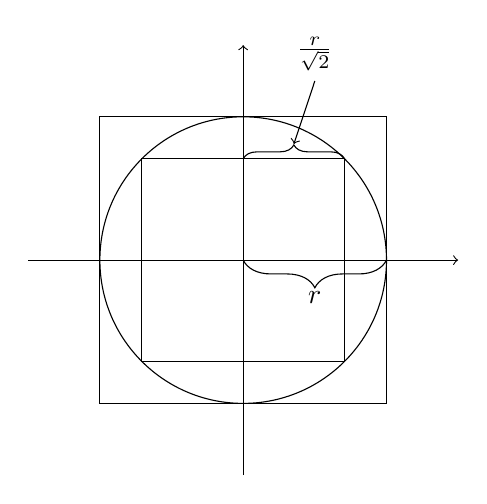
\begin{tikzpicture}[scale=0.91]
\draw[->](-3,0) -- (3,0);
\draw[->](0,-3) -- (0,3);
\draw (-2,-2) rectangle (2,2);
\draw (0,0) circle (2);
\draw (-{sqrt(2)},-{sqrt(2)}) rectangle ({sqrt(2)},{sqrt(2)});
\draw [decorate,decoration={brace,amplitude=10pt}]
(2,0) -- (0,0);
\draw (1,-0.3) node[anchor=north]{$r$};
\draw [decorate,decoration={brace,amplitude=5pt}]
(0,{sqrt(2)}) -- ({sqrt(2)},{sqrt(2)});
\draw[->](1,2.5) -- ({sqrt(2)/2},1.62);
\draw (1,2.5) node[anchor=south]{$\frac{r}{\sqrt{2}}$};
\end{tikzpicture}
\end{center}

\[{\left( { - \frac{r}{{\sqrt 2 }},\frac{r}{{\sqrt 2 }}} \right)^2} \subset {B_{ \le r}}\left( 0 \right) \subset {\left( { - r,r} \right)^2}\]

\begin{beweis}{von Satz 3.28}
\begin{enumerate}[align=left]
\item[(i)$\Rightarrow$(ii)]Folgt aus der Ungleichung $\abs{ {a_n^{(i)} - {a^{(i)}}} } \le \left\| {{a_n} - a} \right\|$
\item[(ii)$\Rightarrow$(i)]Sei $a^i=\lim a_n^i$ und $a=\left( a^i\right)_i$. Aus \[\left\| {{a_n} - a} \right\| \le \sqrt d \mathop {\max }\limits_{1 \le i \le d} \abs{ {a_n^{(i)} - {a^{(i)}}} }\] folgt (i)
\end{enumerate}
\end{beweis}

\subsubsection*{Satz 3.29 (Bolzano - Weierstrasse)}
Jede beschränkte Folge $\left( a_n\right)_{n\geq 1}$ in $\R^d$ besitzt eine konvergente Teilfolge
\subsubsection*{Beispiel}
\begin{enumerate}
\item\begin{align*} ({a_n}) &= \left( {\begin{array}{*{20}{c}}
{{\raise0.7ex\hbox{$1$} \!\mathord{\left/
{\vphantom {1 n}}\right.\kern-\nulldelimiterspace}
\!\lower0.7ex\hbox{$n$}}}\\
{{\raise0.7ex\hbox{$2$} \!\mathord{\left/
{\vphantom {2 n}}\right.\kern-\nulldelimiterspace}
\!\lower0.7ex\hbox{$n$}}}
\end{array}} \right) \subset\R^2 \\
\lim{a_n}&={0 \choose 0} \end{align*}
\item \[ ({a_n}) = {\frac{{n^2} + n + 1}{2{n^2} + n + 1} \choose n} \]
$\left( a_n\right)$ ist divergent
\[\lim \frac{{{n^2} + n + 1}}{{2{n^2} + n + 1}} \to \frac{1}{2}\] aber $\lim n=\infty$
\end{enumerate}

\begin{definition}{3.30}
$\left( a_n\right)_{n\geq 1}$ ist eine Cauchy-Folge falls es $\forall\varepsilon >0$ ein $N(\varepsilon)\geq 1$ gibt, so dass
\[\left\| {{a_n} - {a_m}} \right\| < \varepsilon \hspace{10mm}\forall n,m \ge N(\varepsilon )\]
\end{definition}
\noindent Aus den Sätzen 3.28 und 3.22 (Cauchy-Kriterium) folgt
\subsubsection*{Satz 3.31}
Es sind äquivalent
\begin{enumerate}
\item $\left( a_n\right)_{n\geq 1}$ konvergiert
\item $\left( a_n\right)$ ist eine Cauchy-Folge
\end{enumerate}
Für $\C$ haben wir zusätzlich, dass sich die Körperstruktur mit der Konvergenz gut verträgt. Nämlich
\subsubsection*{Satz 3.32}
Seien $\left( z_n\right)$, $\left( w_n\right)$ zwei konvergente Folgen in $\C$ mit $z=\lim z_n$, $w=\lim w_n$. Dann
\begin{enumerate}[(i)]
\item $\overline{z_n}\to z_n$ und ${\left( {\left\| {{z_n}} \right\|} \right)_{n \ge 1}}$ konvergiert gegen $\norm{z}$
\item Die Folge $\left( z_n w_n\right)_{n\geq 1}$konvergiert gegen $zw$
\item Falls $w\not =0$ und $w_n\not=0$, $\forall n\geq 1$, so konvergiert ${\left( \frac{z_n}{w_n} \right)_{n \ge 1}}$ gegen $\frac{z}{w}$
\end{enumerate}

\section{Reihen}
Sei $\left( a_n\right)_{n\geq 1}$ eine Folge in $\R$ oder $\C$. Sei
\[ S_n:=a_1+a_2+\dots +a_n=\sum\limits_{k = 1}^n {{a_k}} \]
die Folge der partiellen Summen. Eine Reihe ist eine unendliche Summe\[{a_1} + {a_2} +  \ldots  = \sum\limits_{n = 1}^\infty {{a_n}} \] einer Folge $\left( a_n\right)_{n\geq 1}$

\begin{definition}{3.33}
Die Reihe $\sum\limits_{n = 1}^\infty a_n$ ist konvergent, falls die Folge $\left( S_n\right)_{n\geq 1}$ konvergiert. In diesem Fall wird deren Limes mit $\sum\limits_{n = 1}^\infty a_n$ bezeichnet
\[\lim {S_n} = \lim \sum\limits_{k = 1}^n {{a_k}: = \sum\limits_{n = 1}^\infty  {{a_n}} } \]
\end{definition}
\subsubsection*{Beispiel 3.34}
\begin{enumerate}
\item Für $\abs{q}<1$ gilt
\begin{align*}
{S_n}&= \sum\limits_{k = 0}^n {{q^k} = \frac{{1 - {q^{n + 1}}}}{{1 - q}}} \\
\lim {S_n}&= \mathop {\lim }\limits_{n \to \infty } \frac{{1 - {q^{n + 1}}}}{{1 - q}} = \frac{1}{{1 - q}}\text{  (da $\lim q^n=0$)}
\end{align*}
Somit konvergiert $\sum\limits_{k = 1}^\infty  {{q^k}} $ und deren Wert ist $\frac{1}{1-q}$
\item Die Harmonische Reihe $\sum\limits_{n = 1}^\infty  {\frac{1}{n}} $ ist nach Beispiel 3.23 (i) divergent.
\end{enumerate}
Für Reihen gibt es verschiedene praktische Konvergenz-Kriterien. Das erste ergibt sich direkt aus dem Cauchy-Kriterium (Satz 3.22, s.~\pageref{satz3.22})

\subsubsection*{Satz 3.35 (Cauchy-Kriterium)}
Die Reihe $\sum\limits_{n = 1}^\infty  {{a_n}} $ konvergiert genau dann, wenn es für jedes $\varepsilon>0$ einen Index $N(\varepsilon)\geq 1$ gibt,, so dass
\[ \forall n\geq m\geq N(\varepsilon)\hspace{5mm}\abs{ \sum\limits_{k=m}^n a_k}<\varepsilon\]

\begin{beweis}{}
\todo[inline]{It says Übung, maybe incomplete? page 97 top}
Die Reihe $\sum\limits_1^\infty  {{a_j}} $ konvergiert genau dann, wenn
\[\abs{ {\sum\limits_m^n {{a_j}} } } \to 0\hspace{10mm}\forall n \ge m\]
$\sum\limits_1^\infty  {{a_j}} $ konv. $\Leftrightarrow S_n=\sum\limits_1^n a_k$ konv. $\Leftrightarrow S_n$ Cauchy $\Rightarrow \forall\varepsilon>0, \exists N(\varepsilon)$ s.d.
\[\forall n > m > N(\varepsilon)\hspace{10mm}\underbrace {\abs{ {{S_n} - {S_m}} }}_{\sum\limits_m^n {{a_k}} } < \varepsilon \]
\end{beweis}
\subsubsection*{Korollar}
$\sum\limits_{k = 1}^\infty  {{a_k}} $ konvergent $\Rightarrow\abs{ a_k}\to 0$

\begin{beweis}{}
Nehmen wir $m=n$ an in Satz 3.5 (s.\todo{Add Reference. UPDATE: CAN'T FIND SATZ 3.5!!}). Das ist ein notwendiges Kriterium aber nicht ein hinreichendes Kriterium.
\end{beweis}
\todo[inline]{Content between brackets  looks like personal notes, should these be copied? page 97 bottom}

\subsubsection*{Beispiel}
$\sum\limits_1^\infty  k $ ist nicht konvergent, weil $\mathop {\lim }\limits_{k \to \infty } k\not  = 0$ (notwendig).\\
$\sum\frac{1}{k}$ ist nicht konvergent obwohl $\lim\frac{1}{k}=0$ (nicht genügend)\\

Im folgenden leiten wir aus dem Vergleich mit der geometrischen Reihe verschiedene Konvergenz-Kriterien ab (Quotienten- und Wurzelkriterium). Dies stützt sich auf

\subsubsection*{Satz 3.36}\label{satz3.36}
Seien $\sum\limits_1^\infty  {{a_k}} $, $\sum\limits_1^\infty  {{b_k}} $ Reihen wobei
\begin{enumerate}
\item Es gibt $k_0$, so dass $\abs{ a_k} \leq b_k$, $\forall k > k_0$
\item $\sum b_k$ konvergiert
\end{enumerate}
Dann konvergiert $\sum\limits_{k = 1}^\infty  {{a_k}} $

\begin{beweis}{}
Sei $\varepsilon>0$ und $N(\varepsilon) > k_0$, so dass
\[\sum\limits_{k = m}^n {{b_k}}  = \abs{ {\sum\limits_{k = m}^n {{b_k}} } } \le \varepsilon\hspace{10mm} \forall n,m > N(\varepsilon ) > {k_0}\]
Dann folgt aus 1.
\[\abs{ {\sum\limits_{k = m}^n {{a_k}} } } \le \sum\limits_{k = m}^n {\abs{ {{a_k}} }}  \le \sum\limits_{k = m}^n {{b_k}}  \le \varepsilon \]
Der Satz folgt aus dem Cauchy-Kriterium
\end{beweis}
\subsubsection*{Beispiel}
\begin{enumerate}
\item \[\sum\limits_{k = 1}^\infty  {\frac{1}{{k!}} = ?} \]
\[\frac{1}{{k!}} \le \frac{1}{{{2^{k - 1}}}}\hspace{5mm}\forall k \ge 1 \Rightarrow \sum\limits_1^\infty  {\frac{1}{{k!}} < } \sum\limits_1^\infty  {\frac{1}{{{2^{k - 1}}}}}  = 2\]
\item \[\sum\limits_{k = 1}^\infty  {\frac{1}{{{{\left( {k + 1} \right)}^2}}} = ?} \]
Zuerst zeigen wir, dass $\sum\limits_1^\infty  {\frac{1}{{k\left( {k + 1} \right)}}} $ konvergiert. Da
\begin{align*}
\frac{1}{{k\left( {k + 1} \right)}}&= \frac{1}{k} - \frac{1}{{k + 1}}\hspace{10mm}\forall k \ge 1\\
{S_n} = \sum\limits_1^\infty  {\frac{1}{{k\left( {k + 1} \right)}}} &= \left( {1 - \frac{1}{2}} \right) + \left( {\frac{1}{2} - \frac{1}{3}} \right) +  \ldots  + \left( {\frac{1}{{n - 1}} - \frac{1}{n}} \right)\\
&= 1 - \frac{1}{n}
\end{align*}
$\mathop {\lim }\limits_{n \to \infty } {S_n} = 1,{\text{ d.h. }}\sum\limits_1^\infty  {\frac{1}{{k\left( {k + 1} \right)}} = 1} {\text{ }}$.\\
$\forall k > 1$ Da
\begin{align*}
{\left( {k + 1} \right)^2} > k\left( {k + 1} \right)\\
\frac{1}{{{{\left( {k + 1} \right)}^2}}} < \frac{1}{{k\left( {k + 1} \right)}}
\end{align*}
Daraus folgt
\[\sum {\frac{1}{{{{\left( {k + 1} \right)}^2}}}}  \le \sum {\frac{1}{{k\left( {k + 1} \right)}}}  = 1\]
$\sum {\frac{1}{{{{\left( {k + 1} \right)}^2}}}} $ konvergiert.
\end{enumerate}

\subsubsection*{Satz 3.37 (Quotientenkriterium)}
Sei $a_k\not=0$, $\forall k\geq 1$

\begin{enumerate}[(i)]
\item \label{satz3.37}Falls \[\mathop {\lim }\limits_{k \to \infty } \sup \abs{ {\frac{{{a_{k + 1}}}}{{{a_k}}}} } < 1\] so ist $\sum a_k$ konvergent
\item Falls \[\mathop {\lim }\limits_{k \to \infty } \inf \abs{ {\frac{{{a_{k + 1}}}}{{{a_k}}}} } > 1\] so ist $\sum a_k$ divergent
\end{enumerate}

\begin{beweis}{}
\begin{enumerate}[(i)]
\item Sei ${q_0}: = \lim \sup \abs{ {\frac{{{a_{k + 1}}}}{{{a_k}}}} }$ \[\mathop {\lim }\limits_{k \to \infty } \left( {\sup \abs{ {\frac{{{a_{k + 1}}}}{{{a_k}}}} }} \right) = \mathop {\lim }\limits_{n \to \infty } \left( {\mathop {\sup }\limits_{k \ge n} \abs{ {\frac{{{a_{k + 1}}}}{{{a_k}}}} }} \right)\]
Wähle $q\in\R$ mit $q_0<q<1$. Dann gilt für genügend grosse $n_0\in\N$
\begin{align*}
\forall n \ge {n_0}:&\left| {\mathop {\sup }\limits_{k \ge n} \abs{ {\frac{{{a_{k + 1}}}}{{{a_k}}}} } - {q_0}} \right| \le \underbrace {\left( {q - {q_0}} \right)}_\varepsilon\\
{\text{d.h. }}&\text{ }\mathop {\sup }\limits_{k \ge n} \abs{ {\frac{{{a_{k + 1}}}}{{{a_k}}}} } \le q\hspace{5mm}\forall n \ge {n_0}
\end{align*}
Insbesondere bei der Wahl von $n=n_0$
\[\forall k \ge {n_0}\hspace{10mm}\abs{ {\frac{{{a_{k + 1}}}}{{{a_k}}}} } \le q\]
Es folgt für $k\geq n_0$ die Abschätzung
\begin{align*}
\abs{ {{a_k}} }&= \abs{ {\frac{{{a_k}}}{{{a_{k - 1}}}} \cdot \frac{{{a_{k - 1}}}}{{{a_{k - 2}}}} \cdot  \ldots  \cdot \frac{{{a_{{n_0} + 1}}}}{{{a_{{n_0}}}}} \cdot {a_{{n_0}}}} }\\
&\le {q^{k - {n_0}}}\abs{ {{a_{{n_0}}}} } = \underbrace {{q^n}\abs{ {{a_{{n_0}}}} }}_C{q^k} = C{q^k}
\end{align*}
Wir können nun $b_k=Cq^k$ setzen und Satz 3.36 (s.~\pageref{satz3.36}) anwenden. Da $\sum b_k$ konvergiert (da $\abs{ q} < 1$), konvergiert $\sum a_k$.
\item Sei
\[{q_0}: = \mathop {\lim }\limits_{k \to \infty } \inf \abs{ {\frac{{{a_{k + 1}}}}{{{a_k}}}} } = \mathop {\lim }\limits_{n \to \infty } \mathop {\inf }\limits_{k \ge n} \abs{ {\frac{{{a_{k + 1}}}}{{{a_k}}}} }\]
(falls es existiert). Wähle $q\in\R$ mit $q_0>q>1$. Dann existiert $n_0$ mit \[\forall k > {n_0}:\abs{ {\frac{{{a_{k + 1}}}}{{{a_k}}}} } > \mathop {\inf }\limits_{k > {n_0}} \abs{ {\frac{{{a_{k + 1}}}}{{{a_k}}}} } \ge q\]
\[\left( \begin{array}{l}
\hspace{4mm}\left| {\mathop {\inf }\limits_{k \ge n} \abs{ {\frac{{{a_{k + 1}}}}{{{a_k}}}} } - {q_0}} \right| < \underbrace {q - {q_0}}_\varepsilon \hspace{4mm}\forall k > {n_0}\\
 \Rightarrow  - {q_0} + q < \inf \abs{ {\frac{{{a_{k + 1}}}}{{{a_k}}}} } - {q_0}\hspace{5mm}\forall k > {n_0}
\end{array} \right)\]
Dann folgt analog wie in (i), dass
\begin{align*}
\abs{ {{a_k}} }&= \abs{ {\frac{{{a_k}}}{{{a_{k - 1}}}} \cdot \frac{{{a_{k - 1}}}}{{{a_{k - 2}}}} \cdot  \ldots  \cdot \frac{{{a_{{n_0} + 1}}}}{{{a_{{n_0}}}}} \cdot {a_{{n_0}}}} }\\
&> {q^{k - {n_0}}}\abs{ {{a_{{n_0}}}} } > C{q^k}, \forall k>k_0
\end{align*}
Insbesondere ist $\left\{ {\abs{ {{a_k}} }:k \ge 1} \right\}$ nicht beschränkt $\Rightarrow$ $\lim a_k\not\to 0\Rightarrow\sum a_k$ divergent.\\
Falls $\lim \abs{ {\frac{{{a_{k + 1}}}}{{{a_k}}}} }$ existiert, dann \[\lim \inf \abs{ {\frac{{{a_{k + 1}}}}{{{a_k}}}} } = \lim \sup \abs{ {\frac{{{a_{k + 1}}}}{{{a_k}}}} } = \lim \abs{ {\frac{{{a_{k + 1}}}}{{{a_k}}}} } = L\]
\end{enumerate}
\end{beweis}

\subsubsection*{Satz 3.36'}
Sei $a_k\not=0$, $\forall k\in\N$ und sei $L = \mathop {\lim }\limits_{k \to \infty } \abs{ {\frac{{{a_{k + 1}}}}{{{a_k}}}} }$
\begin{enumerate}[(i)]
\item Falls $L<1$, so ist $\sum a_k$ konvergent
\item Falls $L>1$, so ist $\sum a_k$ divergent
\item Falls $L=1$, kann man daraus nichts ableiten
\end{enumerate}
\subsubsection*{Beispiel}
\begin{enumerate}
\item $\sum\limits_1^\infty  {\frac{{n!}}{{{n^n}}}} $ konvergiert. Da
\begin{align*}
\abs{ {\frac{{(n + 1)!}}{{{{\left( {n + 1} \right)}^{n + 1}}}} \cdot \frac{{{n^n}}}{{n!}}} }&= \left( {n + 1} \right) \cdot \frac{{{n^n}}}{{{{\left( {n + 1} \right)}^{n + 1}}}} = {\left( {\frac{n}{{n + 1}}} \right)^n}\\
&={\left( {\frac{1}{{1 + \frac{1}{n}}}} \right)^n} \to \frac{1}{e} < 1
\end{align*}
Insbesondere $\frac{n!}{n^n}\to 0$ falls $n\to\infty$, d.h. $n^n$ wächst schneller als $n!$ (schon gesehen). \todo{Maybe add where?? page 104 top}
\item Wir haben schon gesehen, dass $\sum\frac{1}{n^2}$ konvergiert. Aber Quotientenkriterium gibt keine Information, dass \[\abs{ {\frac{{{a_{n + 1}}}}{{{a_n}}}} } = \abs{ {\frac{{{{\left( {n + 1} \right)}^2}}}{{{n^2}}}} } \to 1\]
\item Wir haben auch schon gesehen dass $\sum\frac{1}{n}$ divergiert. In diesem fall auch \[\abs{ {\frac{{{a_{n + 1}}}}{{{a_n}}}} } = {\frac{{{{ {k + 1} }}}}{{{k}}}}  \to 1\] d.h. das Quotientenkriterium ist nicht anwendbar.
\item Exponentialreihen
\[\exp(z):=\sum\limits_{k=0}^\infty\frac{z^k}{k!}\]
konvergiert für jedes $z\in\C$. Sei $a_k:=\frac{z^k}{k!}$.
\[\frac{{{a_{k + 1}}}}{{{a_k}}} = \frac{{{z^{k + 1}}}}{{\left( {k + 1} \right)!}} \cdot \frac{{k!}}{{{z^k}}} = \frac{z}{{k + 1}}\]
Also
\[\mathop {\lim }\limits_{k \to \infty } \abs{ {\frac{{{a_{k + 1}}}}{{{a_k}}}} } = \mathop {\lim }\limits_{k \to \infty } \abs{ {\frac{z}{{k + 1}}} } = 0 < 1\hspace{5mm}\forall z \in\C \]
Nach Satz 3.37 (i) (s.~\pageref{satz3.37}) ist $\sum {\frac{{{z^k}}}{{k!}}} $ konvergent. Wir werden darauf züruckkommen.
\item Bestimme, für welche $z\in\C$ konvergiert \[\sum\limits_{k = 1}^\infty  {\frac{{{z^k}k!}}{{{k^k}}}} \]
Sei ${a_n} = \frac{{{z^k}k!}}{{{k^k}}}$
\begin{align*}
\frac{{{a_{k + 1}}}}{{{a_k}}}&= \frac{{{z^{k + 1}}\left( {k + 1} \right)!}}{{{{\left( {k + 1} \right)}^{k + 1}}}} \cdot \frac{{{k^k}}}{{k!{z^k}}}\\
&= z\frac{{\left( {k + 1} \right)}}{{\left( {k + 1} \right)}}{\left( {\frac{k}{{k + 1}}} \right)^k} = z\frac{1}{{{{\left( {1 + \frac{1}{k}} \right)}^k}}}
\end{align*}
Dann ist $\lim\abs{\frac{a_{k+1}}{a_k}}=\frac{\abs{z}}{e}$.
Somit folgt die Konvergenz für $\abs{z}<e$ und die Divergenz für $\abs{z}>e$. $\abs{z}<e$ ist der ``Konvergenzkreis'' für $\sum {\frac{{{z^k}k!}}{{{k^k}}}} $
\end{enumerate}
Beispiele 4., 5. sind die erste Einführung des Begriffs des Konvergenzkreises. Das Quotientenkriterium versagt, wenn unendlich viele $a_k$ verschwinden oder falls $\lim\abs{\frac{a_{k+1}}{a_k}}=1$
\subsubsection*{Satz 3.39 (Wurzelkriterium)}\label{satz3.39}
Sei $\left( a_n\right)_{n\geq 1}$ eine Folge in $\R$ oder $\C$
\begin{enumerate}[(i)]
\item Falls $\lim\sup\sqrt[k]{\abs{a_k}}<1$, so konvergiert $\sum\limits_1^\infty a_k$
\item Falls $\lim\sup\sqrt[k]{\abs{a_k}}>1$, so divergiert $\sum\limits_1^\infty a_k$
\end{enumerate}

\begin{beweis}{}
\todo[inline]{Ask for full beweis}
\end{beweis}

\subsubsection*{Beispiel}
\[\sum {{{\left( {\frac{n}{{n + 1}}} \right)}^{{n^2}}}} \] konvergiert, da
\[{\left( {{{\left( {\frac{n}{{n + 1}}} \right)}^{{n^2}}}} \right)^{\frac{1}{n}}} = {\left( {\frac{n}{{n + 1}}} \right)^n} = \frac{1}{{{{\left( {1 + \frac{1}{n}} \right)}^n}}} = \frac{1}{e} < 1\]
Der letzte Satz ist sehr fundamental im Studium der Potenzreihen. Potenzreihen sind wichtig, weil sie analytische Funktionen darstellen.

\begin{definition}{}
Sei $\left( c_k\right)_{k\in\N}$ eine Folge in $\R$ oder $\C$. Betrachte die Potenzreihe in $z\in\C$ \[p(z): = \sum\limits_{k = 0}^\infty  {{c_k}{z^k}} \]
\end{definition}
Mit Satz 3.39 (Wurzelkriterium, s.~\pageref{satz3.39}) erhalten wir die folgende Charakterisierung des Konvergenzbereichs von $p(z)$
\subsubsection*{Satz 3.40}
Die Potenzreihe \[p(z): = \sum\limits_{k = 0}^\infty  {{c_k}{z^k}} \] ist konvergent $\forall z\in\C$, mit \[\abs{ z } < \rho : = \frac{1}{{\lim \sup \sqrt[k]{{\abs{ {{c_k}} }}}}} \in \left[ {0,\infty } \right]\] Sie ist divergent für alle $\abs{z}>\rho$\\

\noindent\underline{Konvention:} Falls $\left\{ \sqrt[k]{\abs{c_k}},k>1\right\}$ \underline{nicht} beschränkt ist, setzen wir
\[\lim \sup \sqrt[k]{{\abs{ {{c_k}} }}} =  + \infty {\text{  und  }}\rho  = 0\]
Falls $\left\{ \sqrt[k]{\abs{c_k}},k\geq 1\right\}$ beschränkt ist und zudem $\lim \sup \sqrt[k]{{\abs{ {{c_k}} }}} =0$, setzen wir $\rho= +\infty$ d.h. die Reihe $\rho(z)$ konvergiert für alle $z\in\C$.

\subsubsection*{Bemerkung}
Insbesondere ist der Konvergenzbereich von $p(z)$ ein Kreis

\subsubsection*{Beispiel 3.41}
Sei \[{c_k} = \left\{ {\begin{array}{*{20}{c}}
1&{k{\text{ gerade}}}\\
{\frac{1}{k}}&{k{\text{ ungerade}}}
\end{array}} \right.\]
Dann gilt \[\frac{{{c_{k + 1}}{z^{k + 1}}}}{{{c_k}{z^k}}} = \left\{ {\begin{array}{*{20}{c}}
{\frac{z}{{\left( {k + 1} \right)}}}&{k{\text{ gerade}}}\\
{zk}&{k{\text{ ungerade}}}
\end{array}} \right.\]
\begin{align*}
\lim \inf \abs{ {\frac{{{c_{k + 1}}{z^{k + 1}}}}{{{c_k}{z^k}}}} }&= \abs{ z }\left( {\lim \inf {a_k}} \right){\text{ mit }}{a_k} = \left\{ {\begin{array}{*{20}{c}}
{\frac{1}{{(k + 1)}}}\\
k
\end{array}} \right.\\
&= \abs{ z }\mathop {\lim }\limits_k \mathop {\inf }\limits_{n \ge k} {a_n} = 0 < 1
\end{align*}
und
\[\abs{ z }\lim \sup \abs{ {\frac{{{c_{k + 1}}}}{{{c_k}}}} } = \abs{ z }\lim \sup {a_k} = \abs{ z }k\]
unbeschränkt für $\abs{z}\not=0$. Das Quotientenkriterium gibt also keine Information. Das Wurzelkriterium dagegen gibt
\[\abs{ z }\sqrt[k]{{\abs{ {{c_k}} }}} = \abs{ k }\left\{ {\begin{array}{*{20}{c}}
1&{k{\text{ gerade}}}\\
{\frac{1}{{\sqrt[k]{k}}}}&{k{\text{ ungerade}}}
\end{array}} \right.\]
Also
\[\rho  = \lim \sqrt[k]{{\abs{ {{c_k}} }}} = 1{\text{  }}\left( {\mathop {\lim }\limits_{n \to \infty } \sqrt[n]{n} = 1} \right)\]
Somit konvergiert $\sum c_kz^k$ für $\abs{z}<1$ und divergiert für $\abs{z}>1$.

\subsubsection*{Bemerkung}
Das Wurzelkriterium ist ``stärker'' als das Quotientenkriterium.

\subsection*{Quotientenkriterium vs. Wurzelkriterium}

\subsubsection*{Lemma }
Sei $\left( a_n\right) \subset\R$ eine Folge. Dann
\[\lim \inf \abs{ {\frac{{{a_{n + 1}}}}{{{a_n}}}} }\mathop  \le \limits_{\mycirc{3}} \lim \inf {\abs{ {{a_n}} }^{\frac{1}{n}}}\mathop  \le \limits_{\mycirc{1}} \lim \sup {\abs{ {{a_n}} }^{\frac{1}{n}}}\mathop  \le \limits_{\mycirc{2}} \lim \sup \abs{ {\frac{{{a_{n + 1}}}}{{{a_n}}}} }\]
\begin{beweis}{}
\begin{enumerate}
\item $\lim \inf {\abs{ {{a_n}} }^{\frac{1}{n}}} \le \lim \sup {\abs{ {{a_n}} }^{\frac{1}{n}}}$ gilt immer
\item Sei $\sigma  = \lim \sup \sqrt[n]{{\abs{ {{a_n}} }}}$, ${q_0} = \lim \sup \abs{ {\frac{{{a_{n + 1}}}}{{{a_n}}}} }$. Wir möchten zeigen, dass $\sigma \leq q_0$. Sei $q>q_0$. $\exists n_0$ genügend gross, so dass
\[\abs{ {\frac{{{a_{n + 1}}}}{{{a_n}}}} } < q\hspace{5mm}\forall n > {n_0}\hspace{5mm}\left(\text{wie im Beweis des Quot. krit}\right)\]
Dann
\begin{align*}
\abs{ {{a_{n + k}}} } &\le \abs{ {\frac{{{a_{n + k}}}}{{{a_{n + k - 1}}}}} }\abs{ {\frac{{{a_{n + k - 1}}}}{{{a_{n + k - 2}}}}} } \ldots \abs{ {\frac{{{a_{n + 1}}}}{{{a_n}}}} }\abs{ {{a_n}} }\\
 &\le {q^k}\abs{ {{a_n}} } = {q^{n + k}}\frac{{\abs{ {{a_n}} }}}{{{q^n}}}\\
 \Rightarrow \abs{ {{a_{n + k}}} } &\le {q^{n + k}}\abs{ {\frac{{{a_n}}}{{{q^n}}}} }\\
 \Rightarrow a_{n + k}^{\frac{1}{{n + k}}} &\le q{\abs{ {\frac{{{a_n}}}{{{q^n}}}} }^{\frac{1}{{n + k}}}}\hspace{5mm}\forall n \ge {n_0}
\end{align*}
Für beliebige $n$ ($n$ ist fix), gilt
\[\mathop {\lim }\limits_{k \to \infty } {\abs{ {\frac{{{a_n}}}{{{q^n}}}} }^{\frac{1}{{n + k}}}} = 1 \Rightarrow \lim \sup a_k^{\frac{1}{k}} \le q \cdot 1 \Rightarrow \sigma  \le q \le {q_0}\]
\item ASK FOR BEWEIS\todo{Ask for beweis, page 110.2 middle}
\end{enumerate}
\end{beweis}

\subsubsection*{Korollar}
\begin{enumerate}
\item Wurzelkriterium ist stärker als das Quotientenkriterium, d.h. liefert bei einer Reihe das Quotientenkriterium eine Enstcheidung (d.h. $\lim\sup\abs{ \frac{a_{n+1}}{a_n}}<1$ im Falle der Konvergenz, $\lim\inf\abs{ \frac{a_{n+1}}{a_n}}>1$ im Falle der Divergenz), so liefert auch das Wurzelkriterium eine Entscheidung (d.h. $\lim\sup\sqrt[n]{a_n}<1$ im Fall der Konvergenz, $\lim\inf\sqrt[n]{a_n}>1$ im Fall der Divergenz)
\item Gibt das Wurzelkriterium keine Information $\Rightarrow$ Gibt das Quotientenkriterium keine Information
\[\left( {\lim \sup \sqrt[n]{{{a_n}}} = 1 \Rightarrow \lim \inf \abs{ {\frac{{{a_{n + 1}}}}{{{a_n}}}} } \le 1} \right)\]
\end{enumerate}
\noindent\underline{Frage:} Warum benutzen wir Quotientenkriterium?\\
\noindent\underline{Antwort:} Manchmal ist es einfacher anzuwenden!

\subsubsection*{Bemerkung}
Das Wurzelkriterium liefert eine Entscheidung über die Divergenz auch wenn $\lim\sup\sqrt[n]{\abs{a_n}}>1$, d.h.
\[\lim \sup \sqrt[n]{{{a_n}}} > 1 \Rightarrow \sum {{a_n}} {\text{ divergent}}\]
da
\[\lim \sup \sqrt[n]{{{a_n}}} > 1 \Rightarrow \lim {a_n}\not  = 0\]
\begin{beweis}{}
\[\lim \sup \sqrt[n]{{{a_n}}} > 1 \Rightarrow \forall {k_0} \in \N\mathop {\sup }\limits_{k \ge {k_0}} \sqrt[k]{{\abs{ {{a_k}} }}} > 1\]
$\Rightarrow\forall k_0\in\N$ gibt es dann ein $k\geq k_0$ mit $\sqrt[k]{\abs{a_k}}\geq 1\Rightarrow\abs{a_k}\geq 1\Rightarrow\lim a_k\not=0\Rightarrow\sum a_k$ divergent.\\

D.h., dass das Wurzelkriterium eine Entscheidung über die Divergenz liefert, ist es hinreichend, dass $\lim\sup\sqrt[n]{\abs{a_n}}>1$.
\end{beweis}

\subsubsection*{Beispiel 3.42 (Riemann Zeta Funktion)}
Für $s>0$ betrachten wir die Reihe
\[\xi (s): = 1 + \frac{1}{{{2^s}}} + \frac{1}{{{3^s}}} + \frac{1}{{{4^s}}} +  \ldots  +  + \frac{1}{{{n^s}}} +  \ldots  = \sum\limits_{n = 1}^\infty  {\frac{1}{{{n^s}}}} \]
und Fragen nach Konvergenz
\begin{enumerate}[(i)]
\item Für $0<s\leq 1$ gilt $\frac{1}{{{k^s}}} \ge \frac{1}{k}$ also
\[\sum\limits_{k = 1}^\infty  {\frac{1}{{{k^s}}}}  \ge \sum\limits_{k = 1}^\infty  {\frac{1}{k}}  \to \infty \]
Also für $0<s\leq 1$, ist $\xi(s)$ divergent.
\item Für $s>1$, sei $a_k=\frac{1}{k^s}$. Dann haben wir
\[\frac{{{a_{k + 1}}}}{{{a_k}}} = {\left( {\frac{k}{{k + 1}}} \right)^s} \to 1\]
und \[\sqrt[k]{{{a_k}}} = \frac{1}{{{{\left( {{k^{\frac{1}{k}}}} \right)}^s}}} \to 1\]
Also funktionieren weder Quotientenkriterium nach Wurzelkriterium.
\end{enumerate}
Wir wenden die Idee an, die zur \todo{Can't read character, page 112 top} Divergenz von $\sum\frac{1}{k}$ führt, jedoch ein wenig modifiziert. Wir hatten (für die Harmonische Reihe)

\begin{align*}
&1 + \underbrace {\frac{1}{2} + \frac{1}{3}}_{\begin{array}{*{20}{c}}
 > \\
{\frac{1}{4} + \frac{1}{4}}
\end{array}} + \underbrace {\frac{1}{4} + \frac{1}{5} + \frac{1}{6} + \frac{1}{7}}_{\begin{array}{*{20}{c}}
 > \\
{\frac{1}{8} + \frac{1}{8} + \frac{1}{8} + \frac{1}{8}}
\end{array}} +  \ldots \\
 \ge&1 + \frac{1}{2} + \frac{1}{2} +  \ldots
\end{align*}
Nun sei $s>1$: Wir segmentieren die Reihe auf die selbe Art
\begin{align*}
&1 + \underbrace {\frac{1}{{{2^s}}} + \frac{1}{{{3^s}}}}_{\begin{array}{*{20}{c}}
 > \\
{\frac{1}{{{2^s}}} + \frac{1}{{{2^s}}}}
\end{array}} + \underbrace {\frac{1}{{{4^s}}} + \frac{1}{{{5^s}}} + \frac{1}{{{6^s}}} + \frac{1}{{{7^s}}}}_{\begin{array}{*{20}{c}}
 > \\
{\frac{1}{{{4^s}}} + \frac{1}{{{4^s}}} + \frac{1}{{{4^s}}} + \frac{1}{{{4^s}}}}
\end{array}} +  \ldots \\
=&1 + \frac{1}{{{2^{s - 1}}}} + \frac{{{2^2}}}{{{2^2}s}} + \frac{{{2^3}}}{{{2^3}s}} +  \ldots \\
=&1 + \frac{1}{{{2^{s - 1}}}} + {\left( {\frac{1}{{{2^{s - 1}}}}} \right)^2} + {\left( {\frac{1}{{{2^{s - 1}}}}} \right)^3} +  \ldots \\
=&\frac{1}{{1 - \frac{1}{{{2^{s - 1}}}}}}
\end{align*}
Also konvergent, da $\frac{1}{{{2^{s - 1}}}} < 1$

\section{Absolute Konvergenz von Reihen}
Wir haben schon gesehen, dass
\begin{itemize}
\item $\sum\frac{1}{n}$ nicht konvergent ist
\item $\sum\frac{\left( -1\right)^n}{n}$ konvergent ist
\end{itemize}
Wir können deshalb herleiten, dass
\[\sum a_n\text{ konvergiert }\not\Rightarrow\sum\abs{a_n}\text{ konvergiert}\]

\begin{definition}{3.43}
Die Reihe $\sum\limits_1^\infty  {{a_k}} $ konvergiert absolut, falls die Reihe $\sum\abs{a_k}$ konvergiert
\[ \text{Konv. }\not\Rightarrow\text{ abs. konv.}\]
\end{definition}

\todo[inline]{Is this sentence really needed? ``Warum sind absolut konvergent Reihen gut?'', page 113 middle}

\subsubsection*{Frage}
Wenn wir eine Reihe haben, können wir in sehr unterschiedlichen Weisen summieren? Kommt es auf die Reihenfolge an?
\subsubsection*{Antwort}
Ja! Es kommt auf die Reihenfolge an!

\subsubsection*{Beispiel 3.44}
Die Reihe $\sum\frac{\left( -1\right)^k}{k}$ konvergiert, hingegen ist $\sum\limits_{k=1}^\infty \frac{1}{2k}$ divergent.\\

\noindent Wählt man zu $l\in\N$ den index $k_l$, so dass
\[\sum\limits_{k = 1}^{{k_l}} {\frac{1}{{2k}}}  > l + \sum\limits_{k = 1}^l {\frac{1}{{2k - 1}}} \]
und ordnet man die Folge $\sum\frac{\left( -1\right)^k}{k}$ nun so um, dass auf die ersten $k_j$ positiven Folgengleider jeweils das $j-$te negative Glied folgt, $j\in\N$, dann erhält man für die so umgeordnete harmonische Reihe
\begin{align*}
\sum {\frac{{{{\left( { - 1} \right)}^k}}}{k}}  =& \frac{1}{2} +  \ldots  + \frac{1}{{2{k_1}}} - 1\\
 &\hspace{15mm}\vdots \\
 +& \frac{1}{{2\left( {{k_1} + 1} \right)}} +  \ldots  + \frac{1}{{2{k_1}}} - \frac{1}{3}\\
&\hspace{15mm} \vdots \\
 +& \frac{1}{{2\left( {{k_{l - 1}} + 1} \right)}} +  \ldots  + \frac{1}{{2{k_l}}} - \frac{1}{{2l - 1}}\\
 &\hspace{15mm}\vdots \\
 =& \sum\limits_{l = 1}^\infty  {\underbrace {\left( {\sum\limits_{k = 1}^{{k_l}} {\frac{1}{{2k}}}  - \sum\limits_{k = 1}^l {\frac{1}{{2k - 1}}} } \right)}_{ > l}} \\
 >& \sum\limits_{l = 1}^\infty  l
\end{align*}
d.h. die umgeordnete alternierende harmonische Reihe ist divergent! Der stärkere Konvergenzbegriff, die absolute Konvergenz, schliesst solche pathologische\\ Verhältnisse aus. Falls die Reihe absolut konvergent ist, ist die Konvergenz sehr stabil und sehr robust.
\subsubsection*{Bemerkung 3.45}
\begin{enumerate}
\item Konv. $\not\Rightarrow$ Abs. Konv. Aber Abs. Konv. $\Rightarrow$ konv.
\begin{beweis}{}
$\sum\abs{a_n}$ konv. Sei $b_n=a_n+\abs{a_n}$
\[{b_n} = \left\{ {\begin{array}{*{20}{l}}
0&{{\text{falls }}{a_n} \le 0}\\
{2{a_n} = 2\abs{ {{a_n}} }}&{{\text{falls }}{a_n} \ge 0}
\end{array}} \right.\]
$\Rightarrow 0\leq b_n\leq 2\abs{a_n}\Rightarrow\sum b_n$ konv.\\
$a_n=b_n-\abs{a_n}$ und beide Reihen konv. $\Rightarrow\sum a_n=\sum b_n-\sum\abs{a_n}$ konv.
\end{beweis}
\item Wurzel- und Quotientenkriterium sind Kriterien für absolute Konvergenz.
\item Da \[{S_n}: = \sum\limits_{k = 1}^n {\abs{ {{a_k}} }}  < {S_{n + 1}} = {S_n} + \abs{ {{a_n}} }\] ist, ist die Folge $\left( S_n\right)_{n\geq 1}$ monoton wachsend; Absolute Konvergenz ist somit äquivalent zur Beschänkheit von $\left( S_n\right)_{n\geq 1}$
\item Falls $\sum a_k$ absolut konvergiert, dann konvergiert natürlich auch $\sum\limits_{k = j}^\infty  {\abs{ {{a_n}} }} $ für jedes $j$ und $\forall \varepsilon > 0$, $\exists j(\varepsilon)$, so dass
\[\sum\limits_{k = j}^\infty  {\abs{ {{a_n}} }}  < \varepsilon\hspace{5mm} \forall j > j(\varepsilon )\]
\end{enumerate}
\begin{framed}
\[\text{\underline{Notation:}}\hspace{3mm}\sum\limits_{k = 1}^\infty  {\abs{ {{a_n}} }}  < \infty  = \sum\limits_{k = 1}^\infty  {\abs{ {{a_k}} }} {\text{ konvergiert}}\]\vspace{-2mm}
\end{framed}

\subsubsection*{Satz 3.46}\label{satz3.46}
Sei $\sum\limits_1^\infty  {{a_k}} $ absolut konvergent und $\varphi :\N\to\N$ eine Bijektion. Dann ist auch die ``umgeordnete Reihe'' $\sum\limits_{k = 1}^\infty  {{a_{\varphi (k)}}} $ absolut konvergent mit gleicher Summe.

\begin{beweis}{}
\todo[inline]{It says Übung, maybe want to add something?? page 117 bottom}
Sei $\varepsilon>0$ vorgegeben. Da $\sum\limits_1^\infty  {\abs{ {{a_k}} }} $ konvergiert, gibt es $n_0(\varepsilon)$ mit $\sum\limits_{k = {n_0}}^\infty  {\abs{ {{a_k}} }}  < \varepsilon $. Sei \[n_1(\varepsilon):=\max\left\{ \varphi^{-1}(1),\varphi^{-1}(2),\dots,\varphi^{-1}(n_0)\right\}\]
Falls $k>n_1(\varepsilon)$, dann folgt $\varphi(k)>n_0$ ($\varphi$ injektiv). Also $\forall n,m\geq n_1(\varepsilon)$
\[\abs{ {\sum\limits_{k = m}^n {{a_{\varphi (k)}}} } } \le \sum\limits_{k = m}^n {\abs{ {{a_{\varphi (k)}}} }}  \le \sum\limits_{k = {n_0}}^\infty  {\abs{ {{a_k}} }}  < \varepsilon \]
Insbesondere konvergiert $\sum\limits_{k = 1}^\infty  {{a_{\varphi (k)}}} $ absolut und
\begin{align*}
\abs{ {\sum\limits_{k = 1}^\infty  {{a_k}}  - \sum\limits_{k = 1}^\infty  {{a_{\varphi (k)}}} } } &\le \abs{ {\sum\limits_{k = 1}^{{n_0}} {{a_k}}  - \sum\limits_{k = 1}^{{n_1}} {{a_{\varphi (k)}}} } } + \abs{ {\sum\limits_{{n_1} + 1}^\infty  {{a_{\varphi (k)}}} } } + \abs{ {\sum\limits_{k = {n_0} + 1}^\infty  {{a_k}} } }\\
&\le 3\sum\limits_{k = {n_0}}^\infty  {\abs{ {{a_k}} }}  \le 3\varepsilon
\end{align*}
\end{beweis}

\subsubsection*{Beispiel 3.47}
$\sum\limits_{k = 1}^\infty  {k{q^k}} $ ist für $\abs{ q} < 1$ absolut konvergent (z.B. Quotientenkriterium)

\begin{align*}
\sum\limits_{k = 1}^\infty  {k{q^k}}  = q + {q^2} + {q^3} + {q^4}&\dots\\
 + {q^2} + {q^3} + {q^4}&\dots\\
 + {q^3} + {q^4}&\dots\\
 + {q^4}&\dots\\
 \vdots &
\end{align*}
\begin{align*}
\sum\limits_{k = 1}^\infty  {k{q^k}} &= q\left\{ {1 + q +  \ldots } \right\} + {q^2}\left\{ {1 + q +  \ldots } \right\}\\
&= \underbrace {\left\{ {1 + q +  \ldots } \right\}}_{\frac{1}{{1 - q}}}\underbrace {\left\{ {q + {q^2} +  \ldots } \right\}}_{\frac{q}{{\left( {1 - q} \right)}}} = \frac{q}{{{{\left( {1 - q} \right)}^2}}}\\
&= \sum\limits_{l = 1}^\infty  {\left( {{q^l}\sum\limits_{k = 0}^\infty  {{q^k}} } \right)}  = \sum\limits_{l = 1}^\infty  {{q^l}} \left( {\frac{1}{{1 - q}}} \right) = \left( {\frac{1}{{1 - q}}} \right)\underbrace {\sum\limits_{l = 1}^\infty  {{q^l}} }_{\frac{q}{{1 - q}}}\\
&= \frac{q}{{{{\left( {1 - q} \right)}^2}}}
\end{align*}
Umordnung der Summation: Statt $\downarrow$ wird $\to$ summiert

\subsubsection*{Satz 3.47}
Seien $\left( a_n\right)_{n\geq 1}$, $\left( b_n\right)_{n\geq 1}$ Folgen in $\R$ oder $\C$. Wir betrachten $\left( a_n b_k\right)_{(n,k)\in\N\times\N}$ als Folge, wobei wir eine beliebige Abzählung von $\N\times\N$ durch $\N$ zulassen. Falls $\sum a_k$, $\sum b_k$ absolut konvergiert, ist $\sum a_k b_k$ absolut konvergent und
\[\sum\limits_{k,l = 1}^\infty  {{a_k}{b_k}}  = \sum\limits_{k = 1}^\infty  {{a_k}} \sum\limits_{l = 1}^\infty  {{b_l}} \]
unabhängig von der Summationsreihenfolge. Als Korollar:

\subsubsection*{Korollar 3.48}
Für alle $x,y$ in $\R$ oder $\C$ gilt
\[ \exp\left( x+y\right)=\exp(x)\exp(y)\]
$\left( \exp(x):=\sum\limits_{k=0}^\infty \frac{x^k}{k!}\right)$

\begin{beweis}{}
\[\exp (x)\exp (y)\mathop  = \limits^{{\text{Satz 3.47}}} \sum\limits_{k\not  = l = 0}^\infty  {\frac{{{x^k}{y^l}}}{{k!l!}}} \]
\begin{center}
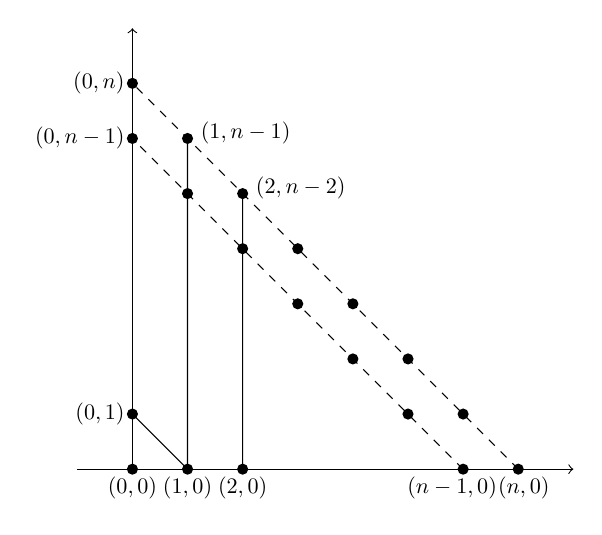
\begin{tikzpicture}[scale=0.7]
\draw[->](-1,0) -- (8,0);
\draw[->](0,0) -- (0,8);
\node[circle,fill=black,inner sep=0.5mm] (a) at (0,0) {} ;
\node[circle,fill=black,inner sep=0.5mm] (a) at (1,0) {} ;
\node[circle,fill=black,inner sep=0.5mm] (a) at (1,6) {} ;
\node[circle,fill=black,inner sep=0.5mm] (a) at (2,5) {} ;
\node[circle,fill=black,inner sep=0.5mm] (a) at (1,5) {} ;
\node[circle,fill=black,inner sep=0.5mm] (a) at (2,4) {} ;
\node[circle,fill=black,inner sep=0.5mm] (a) at (3,4) {} ;
\node[circle,fill=black,inner sep=0.5mm] (a) at (3,3) {} ;
\node[circle,fill=black,inner sep=0.5mm] (a) at (4,3) {} ;
\node[circle,fill=black,inner sep=0.5mm] (a) at (4,2) {} ;
\node[circle,fill=black,inner sep=0.5mm] (a) at (5,2) {} ;
\node[circle,fill=black,inner sep=0.5mm] (a) at (6,1) {} ;
\node[circle,fill=black,inner sep=0.5mm] (a) at (5,1) {} ;
\node[circle,fill=black,inner sep=0.5mm] (a) at (6,0) {} ;
\node[circle,fill=black,inner sep=0.5mm] (a) at (2,0) {} ;
\node[circle,fill=black,inner sep=0.5mm] (a) at (7,0) {} ;
\node[circle,fill=black,inner sep=0.5mm] (a) at (0,1) {} ;
\node[circle,fill=black,inner sep=0.5mm] (a) at (0,7) {} ;
\node[circle,fill=black,inner sep=0.5mm] (a) at (0,6) {} ;
\draw[](1,0) -- (0,1)
(1,0)--(1,6)
(2,0)--(2,5);
\draw[dashed](7,0) -- (0,7)
(6,0) -- (0,6);
%y-axis
\draw (0,6) node[scale=0.8,anchor=east]{$(0,n-1)$};
\draw (0,7) node[scale=0.8,anchor=east]{$(0,n)$};
\draw (0,1) node[scale=0.8,anchor=east]{$(0,1)$};
%x-axis
\draw (0,0) node[scale=0.8,anchor=north]{$(0,0)$};
\draw (1,0) node[scale=0.8,anchor=north]{$(1,0)$};
\draw (2,0) node[scale=0.8,anchor=north]{$(2,0)$};
\draw (5.8,0) node[scale=0.8,anchor=north]{$(n-1,0)$};
\draw (7.1,0) node[scale=0.8,anchor=north]{$(n,0)$};
%middle of the graph
\draw (1.1,6.1) node[scale=0.8,anchor=west]{$(1,n-1)$};
\draw (2.1,5.1) node[scale=0.8,anchor=west]{$(2,n-2)$};
\end{tikzpicture}
\end{center}
Wir zählen jetzt $\N\times\N$ wie folgt ab
\todo[inline]{Can't understand the formula, page 121 bottom}
\[\exp (x)\exp (y) = \sum\limits_{n = 0}^\infty  {\frac{{{{\left( {x + y} \right)}^n}}}{{n!}}}  = \exp \left( {x + y} \right)\]
\end{beweis}
Zum Abschluss behandeln wir noch den Zusammenhang von ``$e$'' und ``$e^x$''.

\subsubsection*{Satz 3.49}
\[\exp\left(1\right)=\mathop {\lim }\limits_{n \to \infty } {\left( {1 + \frac{1}{n}} \right)^n} = e\]

\begin{beweis}{}
\begin{enumerate}
\item \[\exp \left( 1 \right) = \sum\limits_{k = 0}^\infty  {\frac{1}{{k!}}} \]
\begin{align*}
&\Rightarrow\forall\varepsilon >0, \exists n_0=n_0(\varepsilon),\text{mit }\abs{ {\exp \left( 1 \right) - \sum\limits_{k = 0}^\infty  {\frac{1}{{k!}}}  < \varepsilon } }\\
&\Leftrightarrow - \varepsilon  < \sum\limits_0^{{n_0}} {\frac{1}{{k!}}}  - \exp \left( 1 \right) < \varepsilon \\
&\Leftrightarrow  - \varepsilon  + \exp \left( 1 \right) < \sum\limits_0^{n_0} {\frac{1}{{k!}}}  < \varepsilon  + \exp \left( 1 \right)
\end{align*}
Insbesondere
\[\exp \left( 1 \right) < \sum\limits_{k = 0}^{{n_0}} {\frac{1}{{k!}}}  + \varepsilon \]
\item\begin{align*}
{\left( {1 + \frac{1}{n}} \right)^n}& =\sum\limits_{k = 0}^n {n \choose k } \frac{1}{{{n^k}}}\\
& =\sum\limits_{k = 0}^n {\frac{{n!}}{{k!\left( {n - k} \right)!}}}  \cdot \frac{1}{{{n^k}}}\\
&\mathop  =\limits^{(\text{\textasteriskcentered})} \sum\limits_{k = 0}^n {\frac{1}{{k!}}} \underbrace {\left( {\frac{{n\left( {n - 1} \right) \ldots \left( {n - k + 1} \right)}}{{{n^k}}}} \right)}_{a_k^{(n)}}\\
 &=\sum\limits_{k = 0}^n {\frac{1}{{k!}}} a_k^{(n)}
\end{align*}
Da
\[a_k^{(n)}:=\frac{n}{n}\cdot\frac{\left( n-1\right)}{n}\dots\frac{n-k+1}{n}<1\]
\[{\left( {1 + \frac{1}{n}} \right)^n} < \sum\limits_{k = 0}^n {\frac{1}{{k!}}}  < \exp \left( 1 \right) \Rightarrow 0 < \exp \left( 1 \right) - {\left( {1 + \frac{1}{n}} \right)^n}\]
\item $0<a_k^{(n)}<1$ und für jedes $k$ fest ist $a_k^{(n)}\to 1$, $n\to\infty$.
\[\frac{{n\left( {n - 1} \right) \ldots \left( {n - k + 1} \right)}}{{{n^k}}} = \frac{{1\left( {1 - \frac{1}{n}} \right)\left( {1 - \frac{2}{n}} \right) \ldots \left( {1 - \frac{k}{n} + \frac{1}{n}} \right)}}{{\frac{{{n^k}}}{{{n^k}}}}}\mathop  \to \limits_{n \to \infty } 1\]
somit
\[ 1-a_k^{(n)}\mathop  \to \limits_{n \to \infty } 0\text{, ($k$ fest)}\]
\[\Rightarrow\sum\limits_{k = 0}^n {\left( {1 - a_k^{(n)}} \right)} \mathop  \to \limits_{n \to \infty } 0\]
$\Rightarrow$ Für $\varepsilon>0$, $\exists n_1=n_1(\varepsilon,n_0)$,, so dass
\[\forall n \ge {n_1}\hspace{5mm}\sum\limits_{k = 0}^{{n_0}} {\left( {1 - a_k^{(n)}} \right)}  < \varepsilon \]
Dann haben wir $\forall n \ge \max \{ {n_0},{n_1}\} $
\begin{align*}
0&\mathop  < \limits^{\mycirc{2}} \exp \left( 1 \right) - {\left( {1 + \frac{1}{n}} \right)^n}\mathop  < \limits^{()} \sum\limits_{k = 0}^{{n_0}} {\frac{1}{{k!}}}  + \varepsilon  - {\left( {1 + \frac{1}{n}} \right)^n}\\
&\mathop  < \limits^{\mycirc{2}(\text{\textasteriskcentered})} \sum\limits_{k = 0}^{{n_0}} {\frac{1}{{k!}}}  + \varepsilon  - \sum\limits_{k = 0}^n {a_k^{(n)}} \frac{1}{{k!}}\\
 &< \sum\limits_{k = 0}^{{n_0}} {\frac{1}{{k!}}}  + \varepsilon  - \sum\limits_{k = 0}^{{n_0}} {a_k^{(n)}} \frac{1}{{k!}}\\
 &= \sum\limits_{k = 0}^{{n_0}} {\frac{1}{{k!}}} \left( {1 - a_k^{(n)}} \right) + \varepsilon \\
& < \sum\limits_{k = 0}^{{n_0}} {\left( {1 - a_k^{(n)}} \right)}  + \varepsilon  < 2\varepsilon \\
 \Rightarrow&\exp \left( 1 \right) = \mathop {\lim }\limits_{n \to \infty } {\left( {1 + \frac{1}{n}} \right)^n}
\end{align*}
\end{enumerate}
\end{beweis}

Analog kann man auch beweisen, dass
\subsubsection*{Satz 3.50}
$\forall x\in\R$
\[\exp(x)=\mathop {\lim }\limits_{n \to \infty } {\left( {1 + \frac{x}{n}} \right)^n}\]
\todo[inline]{Start of additional content, page 125. This has to be reviewed for layout issues (it's pretty much a mess)}
\subsubsection*{Satz}
\[\exp (x) = \sum {\frac{x}{{k!}}}  \Rightarrow \forall \varepsilon  > 0,\exists {n_0}(\varepsilon )\]
\[\forall n > {n_0}\hspace{5mm}\abs{ {\exp (x) - \sum\limits_0^{{n_0}} {\frac{x}{{k!}}} } } < \varepsilon \]
\begin{align*}
& \Leftrightarrow  - \varepsilon  < \sum {\frac{x}{{k!}}}  - \exp (x) < \varepsilon \\
\mycirc{1}& \Leftrightarrow \exp (x) - \varepsilon  < \sum\limits_0^{{n_0}} {\frac{x}{{k!}}}  < \varepsilon  + \exp (x)
\end{align*}
\begin{align*}
\mycirc{2}\hspace{2mm}{\left( {1 + \frac{x}{n}} \right)^n}&= \sum\limits_0^n {n \choose k} \frac{{{x^n}}}{{{n^k}}}\\
 &= \sum\limits_{k = 0}^n {\frac{{n!}}{{k!\left( {n - k} \right)!}} \cdot } \frac{{{x^k}}}{{{n^k}}}\\
 &= \sum\limits_0^n {\frac{1}{{k!}} \cdot \frac{{n!}}{{\left( {n - k} \right)!}}}  \cdot \frac{{{x^k}}}{{{n^k}}}\\
&\mathop  = \limits^{\mycirc{2}} \sum {\frac{1}{{k!}}}  \cdot \underbrace {\frac{{n\left( {n - 1} \right) \ldots \left( {n - k + 1} \right)}}{{{n^k}}}}_{a_k^{(n)}} \cdot {x^k}\\
 &\le \sum\limits_0^n {\frac{{{x^k}}}{{{n^k}}}}  < \exp (x)\\
 \Rightarrow&\exp (x) - {\left( {1 + \frac{x}{n}} \right)^n} > 0\hspace{2mm}\mycirc{2}
\end{align*}
$0<a_k^n<1$ für jedes $k$ fest ist $a_k^{(n)}\to 1$, $n\to\infty$
\[\frac{{n\left( {n - 1} \right) \ldots \left( {n - k + 1} \right)}}{{{n^k}}} = \frac{{1\left( {1 - \frac{1}{n}} \right)\left( {1 - \frac{2}{n}} \right) \ldots \left( {1 - \frac{k}{n} + \frac{1}{n}} \right)}}{{\frac{{{n^k}}}{{{n^k}}}}} \to 1\]
\begin{align*}
&\Rightarrow 1-a_k^{(n)}\to 0, n\to\infty\hspace{5mm}\text{($k$ fest)}\\
&\Rightarrow \sum\limits_{k = 0}^{{n_0}} {\left( {1 - a_k^{(n)}} \right){x^k} \to } 0, n\to\infty\hspace{5mm}\text{($x,k$ fest)}\\
&\Rightarrow\forall\varepsilon >0\hspace{5mm}\exists n_1=n_1\left(\varepsilon, n_0 \right)\hspace{5mm}\forall n>n_1
\end{align*}
\[\sum\limits_{k = 0}^{{n_0}} {\left( {1 - a_k^{(n)}} \right){x^k}}  < \varepsilon \]
Dann $\forall n>\max\{ n_0,n_1\}$
\begin{align*}
0&\mathop  < \limits^{\mycirc{2}} \exp (x) - {\left( {1 + \frac{x}{n}} \right)^n}\mathop  < \limits^{\mycirc{1}} \sum\limits_0^{{n_0}} {\frac{{{x^k}}}{{k!}}}  + \varepsilon  - {\left( {1 + \frac{x}{n}} \right)^n}\\
 &< \sum\limits_0^{{n_0}} {\frac{{{x^k}}}{{k!}}}  + \varepsilon  - \sum\limits_0^{{n_0}} {a_k^n} \frac{{{x^k}}}{{k!}}\\
 &= \sum\limits_0^{{n_0}} {\frac{{(1 - a_k^n)}}{{k!}}} {x^k} + \varepsilon  < \sum\limits_0^{{n_0}} {\left( {1 - a_k^n} \right)} {x^k} + \varepsilon  < 2\varepsilon
\end{align*}
\todo[inline]{End of additional content}

\noindent Satz 3.49 $\Rightarrow \exp(1)=e^1$
\[\exp \left( {x + y} \right) =\left( {\exp \left( x \right)} \right)\left( {\exp \left( y \right)} \right)\]
\begin{align*}
 \Rightarrow \exp \left( n \right) =&\exp \left( 1 \right)\exp \left( {n - 1} \right)\\
 =&\exp \left( 1 \right)\exp \left( 1 \right)\exp \left( {n - 2} \right)\\
 \vdots \\
 =&e \cdot e \cdot  \ldots  \cdot e = {e^n}, \forall n\in\N
\end{align*}
\[1=\exp(0)=\exp(n)\exp(-n)\]
\[\Rightarrow\exp(-n)=\frac{1}{\exp(n)}=\frac{1}{e^n}=e^{-n}\]
\[\Rightarrow \exp(n)=e^n, \forall n\in\mathbb{Z}\]
\[\forall q\in\N, \exp\left(\frac{1}{q}\right)=e^{\frac{1}{q}}\]
Da
\[ e=\exp(1)=\exp\left(q\cdot\frac{1}{q}\right)=\underbrace {\exp \left( {\frac{1}{q}} \right) \ldots \exp \left( {\frac{1}{q}} \right)}_{q{\text{ mal}}}\]
Somit haben wir
\subsubsection*{Satz 3.51}
$\forall x\in\mathbb{Q}$, $\exp(x)=e^x$. Für rein imaginäre Argumente $z=iy$, $y\in\R$ können wir $\exp(iy)$ durch Umordnung gemäs Satz 3.46 (s.~\pageref{satz3.46}) in Real- und Imaginärteil zerlegen
\begin{align*}
\exp \left( {iy} \right)&= \sum\limits_{k = 0}^\infty  {\frac{{{{\left( {iy} \right)}^k}}}{{k!}}} \\
&= \sum\limits_{l = 0}^\infty  {\frac{{{{\left( { - 1} \right)}^l}{y^{2l}}}}{{\left( {2l} \right)!}}}  + i\sum\limits_{l = 0}^\infty  {\frac{{{{\left( { - 1} \right)}^l}{y^{2l + 1}}}}{{\left( {2l + 1} \right)!}}} \\
&: = \cos \left( y \right) + i\sin \left( y \right)
\end{align*}
Für $z=x+iy\in\C$
\[\exp \left( z \right) = \exp \left( x \right)\exp \left( {iy} \right) = \exp \left( x \right)\left( {\cos \left( y \right) + i\sin \left( y \right)} \right)\]

